
% Default to the notebook output style

    


% Inherit from the specified cell style.




    
\documentclass[11pt]{article}

    
    
    \usepackage[T1]{fontenc}
    % Nicer default font (+ math font) than Computer Modern for most use cases
    \usepackage{mathpazo}

    % Basic figure setup, for now with no caption control since it's done
    % automatically by Pandoc (which extracts ![](path) syntax from Markdown).
    \usepackage{graphicx}
    % We will generate all images so they have a width \maxwidth. This means
    % that they will get their normal width if they fit onto the page, but
    % are scaled down if they would overflow the margins.
    \makeatletter
    \def\maxwidth{\ifdim\Gin@nat@width>\linewidth\linewidth
    \else\Gin@nat@width\fi}
    \makeatother
    \let\Oldincludegraphics\includegraphics
    % Set max figure width to be 80% of text width, for now hardcoded.
    \renewcommand{\includegraphics}[1]{\Oldincludegraphics[width=.8\maxwidth]{#1}}
    % Ensure that by default, figures have no caption (until we provide a
    % proper Figure object with a Caption API and a way to capture that
    % in the conversion process - todo).
    \usepackage{caption}
    \DeclareCaptionLabelFormat{nolabel}{}
    \captionsetup{labelformat=nolabel}

    \usepackage{adjustbox} % Used to constrain images to a maximum size 
    \usepackage{xcolor} % Allow colors to be defined
    \usepackage{enumerate} % Needed for markdown enumerations to work
    \usepackage{geometry} % Used to adjust the document margins
    \usepackage{amsmath} % Equations
    \usepackage{amssymb} % Equations
    \usepackage{textcomp} % defines textquotesingle
    % Hack from http://tex.stackexchange.com/a/47451/13684:
    \AtBeginDocument{%
        \def\PYZsq{\textquotesingle}% Upright quotes in Pygmentized code
    }
    \usepackage{upquote} % Upright quotes for verbatim code
    \usepackage{eurosym} % defines \euro
    \usepackage[mathletters]{ucs} % Extended unicode (utf-8) support
    \usepackage[utf8x]{inputenc} % Allow utf-8 characters in the tex document
    \usepackage{fancyvrb} % verbatim replacement that allows latex
    \usepackage{grffile} % extends the file name processing of package graphics 
                         % to support a larger range 
    % The hyperref package gives us a pdf with properly built
    % internal navigation ('pdf bookmarks' for the table of contents,
    % internal cross-reference links, web links for URLs, etc.)
    \usepackage{hyperref}
    \usepackage{longtable} % longtable support required by pandoc >1.10
    \usepackage{booktabs}  % table support for pandoc > 1.12.2
    \usepackage[inline]{enumitem} % IRkernel/repr support (it uses the enumerate* environment)
    \usepackage[normalem]{ulem} % ulem is needed to support strikethroughs (\sout)
                                % normalem makes italics be italics, not underlines
    

    
    
    % Colors for the hyperref package
    \definecolor{urlcolor}{rgb}{0,.145,.698}
    \definecolor{linkcolor}{rgb}{.71,0.21,0.01}
    \definecolor{citecolor}{rgb}{.12,.54,.11}

    % ANSI colors
    \definecolor{ansi-black}{HTML}{3E424D}
    \definecolor{ansi-black-intense}{HTML}{282C36}
    \definecolor{ansi-red}{HTML}{E75C58}
    \definecolor{ansi-red-intense}{HTML}{B22B31}
    \definecolor{ansi-green}{HTML}{00A250}
    \definecolor{ansi-green-intense}{HTML}{007427}
    \definecolor{ansi-yellow}{HTML}{DDB62B}
    \definecolor{ansi-yellow-intense}{HTML}{B27D12}
    \definecolor{ansi-blue}{HTML}{208FFB}
    \definecolor{ansi-blue-intense}{HTML}{0065CA}
    \definecolor{ansi-magenta}{HTML}{D160C4}
    \definecolor{ansi-magenta-intense}{HTML}{A03196}
    \definecolor{ansi-cyan}{HTML}{60C6C8}
    \definecolor{ansi-cyan-intense}{HTML}{258F8F}
    \definecolor{ansi-white}{HTML}{C5C1B4}
    \definecolor{ansi-white-intense}{HTML}{A1A6B2}

    % commands and environments needed by pandoc snippets
    % extracted from the output of `pandoc -s`
    \providecommand{\tightlist}{%
      \setlength{\itemsep}{0pt}\setlength{\parskip}{0pt}}
    \DefineVerbatimEnvironment{Highlighting}{Verbatim}{commandchars=\\\{\}}
    % Add ',fontsize=\small' for more characters per line
    \newenvironment{Shaded}{}{}
    \newcommand{\KeywordTok}[1]{\textcolor[rgb]{0.00,0.44,0.13}{\textbf{{#1}}}}
    \newcommand{\DataTypeTok}[1]{\textcolor[rgb]{0.56,0.13,0.00}{{#1}}}
    \newcommand{\DecValTok}[1]{\textcolor[rgb]{0.25,0.63,0.44}{{#1}}}
    \newcommand{\BaseNTok}[1]{\textcolor[rgb]{0.25,0.63,0.44}{{#1}}}
    \newcommand{\FloatTok}[1]{\textcolor[rgb]{0.25,0.63,0.44}{{#1}}}
    \newcommand{\CharTok}[1]{\textcolor[rgb]{0.25,0.44,0.63}{{#1}}}
    \newcommand{\StringTok}[1]{\textcolor[rgb]{0.25,0.44,0.63}{{#1}}}
    \newcommand{\CommentTok}[1]{\textcolor[rgb]{0.38,0.63,0.69}{\textit{{#1}}}}
    \newcommand{\OtherTok}[1]{\textcolor[rgb]{0.00,0.44,0.13}{{#1}}}
    \newcommand{\AlertTok}[1]{\textcolor[rgb]{1.00,0.00,0.00}{\textbf{{#1}}}}
    \newcommand{\FunctionTok}[1]{\textcolor[rgb]{0.02,0.16,0.49}{{#1}}}
    \newcommand{\RegionMarkerTok}[1]{{#1}}
    \newcommand{\ErrorTok}[1]{\textcolor[rgb]{1.00,0.00,0.00}{\textbf{{#1}}}}
    \newcommand{\NormalTok}[1]{{#1}}
    
    % Additional commands for more recent versions of Pandoc
    \newcommand{\ConstantTok}[1]{\textcolor[rgb]{0.53,0.00,0.00}{{#1}}}
    \newcommand{\SpecialCharTok}[1]{\textcolor[rgb]{0.25,0.44,0.63}{{#1}}}
    \newcommand{\VerbatimStringTok}[1]{\textcolor[rgb]{0.25,0.44,0.63}{{#1}}}
    \newcommand{\SpecialStringTok}[1]{\textcolor[rgb]{0.73,0.40,0.53}{{#1}}}
    \newcommand{\ImportTok}[1]{{#1}}
    \newcommand{\DocumentationTok}[1]{\textcolor[rgb]{0.73,0.13,0.13}{\textit{{#1}}}}
    \newcommand{\AnnotationTok}[1]{\textcolor[rgb]{0.38,0.63,0.69}{\textbf{\textit{{#1}}}}}
    \newcommand{\CommentVarTok}[1]{\textcolor[rgb]{0.38,0.63,0.69}{\textbf{\textit{{#1}}}}}
    \newcommand{\VariableTok}[1]{\textcolor[rgb]{0.10,0.09,0.49}{{#1}}}
    \newcommand{\ControlFlowTok}[1]{\textcolor[rgb]{0.00,0.44,0.13}{\textbf{{#1}}}}
    \newcommand{\OperatorTok}[1]{\textcolor[rgb]{0.40,0.40,0.40}{{#1}}}
    \newcommand{\BuiltInTok}[1]{{#1}}
    \newcommand{\ExtensionTok}[1]{{#1}}
    \newcommand{\PreprocessorTok}[1]{\textcolor[rgb]{0.74,0.48,0.00}{{#1}}}
    \newcommand{\AttributeTok}[1]{\textcolor[rgb]{0.49,0.56,0.16}{{#1}}}
    \newcommand{\InformationTok}[1]{\textcolor[rgb]{0.38,0.63,0.69}{\textbf{\textit{{#1}}}}}
    \newcommand{\WarningTok}[1]{\textcolor[rgb]{0.38,0.63,0.69}{\textbf{\textit{{#1}}}}}
    
    
    % Define a nice break command that doesn't care if a line doesn't already
    % exist.
    \def\br{\hspace*{\fill} \\* }
    % Math Jax compatability definitions
    \def\gt{>}
    \def\lt{<}
    % Document parameters
    \title{CarND-Object-Detection-Lab}
    
    
    

    % Pygments definitions
    
\makeatletter
\def\PY@reset{\let\PY@it=\relax \let\PY@bf=\relax%
    \let\PY@ul=\relax \let\PY@tc=\relax%
    \let\PY@bc=\relax \let\PY@ff=\relax}
\def\PY@tok#1{\csname PY@tok@#1\endcsname}
\def\PY@toks#1+{\ifx\relax#1\empty\else%
    \PY@tok{#1}\expandafter\PY@toks\fi}
\def\PY@do#1{\PY@bc{\PY@tc{\PY@ul{%
    \PY@it{\PY@bf{\PY@ff{#1}}}}}}}
\def\PY#1#2{\PY@reset\PY@toks#1+\relax+\PY@do{#2}}

\expandafter\def\csname PY@tok@w\endcsname{\def\PY@tc##1{\textcolor[rgb]{0.73,0.73,0.73}{##1}}}
\expandafter\def\csname PY@tok@c\endcsname{\let\PY@it=\textit\def\PY@tc##1{\textcolor[rgb]{0.25,0.50,0.50}{##1}}}
\expandafter\def\csname PY@tok@cp\endcsname{\def\PY@tc##1{\textcolor[rgb]{0.74,0.48,0.00}{##1}}}
\expandafter\def\csname PY@tok@k\endcsname{\let\PY@bf=\textbf\def\PY@tc##1{\textcolor[rgb]{0.00,0.50,0.00}{##1}}}
\expandafter\def\csname PY@tok@kp\endcsname{\def\PY@tc##1{\textcolor[rgb]{0.00,0.50,0.00}{##1}}}
\expandafter\def\csname PY@tok@kt\endcsname{\def\PY@tc##1{\textcolor[rgb]{0.69,0.00,0.25}{##1}}}
\expandafter\def\csname PY@tok@o\endcsname{\def\PY@tc##1{\textcolor[rgb]{0.40,0.40,0.40}{##1}}}
\expandafter\def\csname PY@tok@ow\endcsname{\let\PY@bf=\textbf\def\PY@tc##1{\textcolor[rgb]{0.67,0.13,1.00}{##1}}}
\expandafter\def\csname PY@tok@nb\endcsname{\def\PY@tc##1{\textcolor[rgb]{0.00,0.50,0.00}{##1}}}
\expandafter\def\csname PY@tok@nf\endcsname{\def\PY@tc##1{\textcolor[rgb]{0.00,0.00,1.00}{##1}}}
\expandafter\def\csname PY@tok@nc\endcsname{\let\PY@bf=\textbf\def\PY@tc##1{\textcolor[rgb]{0.00,0.00,1.00}{##1}}}
\expandafter\def\csname PY@tok@nn\endcsname{\let\PY@bf=\textbf\def\PY@tc##1{\textcolor[rgb]{0.00,0.00,1.00}{##1}}}
\expandafter\def\csname PY@tok@ne\endcsname{\let\PY@bf=\textbf\def\PY@tc##1{\textcolor[rgb]{0.82,0.25,0.23}{##1}}}
\expandafter\def\csname PY@tok@nv\endcsname{\def\PY@tc##1{\textcolor[rgb]{0.10,0.09,0.49}{##1}}}
\expandafter\def\csname PY@tok@no\endcsname{\def\PY@tc##1{\textcolor[rgb]{0.53,0.00,0.00}{##1}}}
\expandafter\def\csname PY@tok@nl\endcsname{\def\PY@tc##1{\textcolor[rgb]{0.63,0.63,0.00}{##1}}}
\expandafter\def\csname PY@tok@ni\endcsname{\let\PY@bf=\textbf\def\PY@tc##1{\textcolor[rgb]{0.60,0.60,0.60}{##1}}}
\expandafter\def\csname PY@tok@na\endcsname{\def\PY@tc##1{\textcolor[rgb]{0.49,0.56,0.16}{##1}}}
\expandafter\def\csname PY@tok@nt\endcsname{\let\PY@bf=\textbf\def\PY@tc##1{\textcolor[rgb]{0.00,0.50,0.00}{##1}}}
\expandafter\def\csname PY@tok@nd\endcsname{\def\PY@tc##1{\textcolor[rgb]{0.67,0.13,1.00}{##1}}}
\expandafter\def\csname PY@tok@s\endcsname{\def\PY@tc##1{\textcolor[rgb]{0.73,0.13,0.13}{##1}}}
\expandafter\def\csname PY@tok@sd\endcsname{\let\PY@it=\textit\def\PY@tc##1{\textcolor[rgb]{0.73,0.13,0.13}{##1}}}
\expandafter\def\csname PY@tok@si\endcsname{\let\PY@bf=\textbf\def\PY@tc##1{\textcolor[rgb]{0.73,0.40,0.53}{##1}}}
\expandafter\def\csname PY@tok@se\endcsname{\let\PY@bf=\textbf\def\PY@tc##1{\textcolor[rgb]{0.73,0.40,0.13}{##1}}}
\expandafter\def\csname PY@tok@sr\endcsname{\def\PY@tc##1{\textcolor[rgb]{0.73,0.40,0.53}{##1}}}
\expandafter\def\csname PY@tok@ss\endcsname{\def\PY@tc##1{\textcolor[rgb]{0.10,0.09,0.49}{##1}}}
\expandafter\def\csname PY@tok@sx\endcsname{\def\PY@tc##1{\textcolor[rgb]{0.00,0.50,0.00}{##1}}}
\expandafter\def\csname PY@tok@m\endcsname{\def\PY@tc##1{\textcolor[rgb]{0.40,0.40,0.40}{##1}}}
\expandafter\def\csname PY@tok@gh\endcsname{\let\PY@bf=\textbf\def\PY@tc##1{\textcolor[rgb]{0.00,0.00,0.50}{##1}}}
\expandafter\def\csname PY@tok@gu\endcsname{\let\PY@bf=\textbf\def\PY@tc##1{\textcolor[rgb]{0.50,0.00,0.50}{##1}}}
\expandafter\def\csname PY@tok@gd\endcsname{\def\PY@tc##1{\textcolor[rgb]{0.63,0.00,0.00}{##1}}}
\expandafter\def\csname PY@tok@gi\endcsname{\def\PY@tc##1{\textcolor[rgb]{0.00,0.63,0.00}{##1}}}
\expandafter\def\csname PY@tok@gr\endcsname{\def\PY@tc##1{\textcolor[rgb]{1.00,0.00,0.00}{##1}}}
\expandafter\def\csname PY@tok@ge\endcsname{\let\PY@it=\textit}
\expandafter\def\csname PY@tok@gs\endcsname{\let\PY@bf=\textbf}
\expandafter\def\csname PY@tok@gp\endcsname{\let\PY@bf=\textbf\def\PY@tc##1{\textcolor[rgb]{0.00,0.00,0.50}{##1}}}
\expandafter\def\csname PY@tok@go\endcsname{\def\PY@tc##1{\textcolor[rgb]{0.53,0.53,0.53}{##1}}}
\expandafter\def\csname PY@tok@gt\endcsname{\def\PY@tc##1{\textcolor[rgb]{0.00,0.27,0.87}{##1}}}
\expandafter\def\csname PY@tok@err\endcsname{\def\PY@bc##1{\setlength{\fboxsep}{0pt}\fcolorbox[rgb]{1.00,0.00,0.00}{1,1,1}{\strut ##1}}}
\expandafter\def\csname PY@tok@kc\endcsname{\let\PY@bf=\textbf\def\PY@tc##1{\textcolor[rgb]{0.00,0.50,0.00}{##1}}}
\expandafter\def\csname PY@tok@kd\endcsname{\let\PY@bf=\textbf\def\PY@tc##1{\textcolor[rgb]{0.00,0.50,0.00}{##1}}}
\expandafter\def\csname PY@tok@kn\endcsname{\let\PY@bf=\textbf\def\PY@tc##1{\textcolor[rgb]{0.00,0.50,0.00}{##1}}}
\expandafter\def\csname PY@tok@kr\endcsname{\let\PY@bf=\textbf\def\PY@tc##1{\textcolor[rgb]{0.00,0.50,0.00}{##1}}}
\expandafter\def\csname PY@tok@bp\endcsname{\def\PY@tc##1{\textcolor[rgb]{0.00,0.50,0.00}{##1}}}
\expandafter\def\csname PY@tok@fm\endcsname{\def\PY@tc##1{\textcolor[rgb]{0.00,0.00,1.00}{##1}}}
\expandafter\def\csname PY@tok@vc\endcsname{\def\PY@tc##1{\textcolor[rgb]{0.10,0.09,0.49}{##1}}}
\expandafter\def\csname PY@tok@vg\endcsname{\def\PY@tc##1{\textcolor[rgb]{0.10,0.09,0.49}{##1}}}
\expandafter\def\csname PY@tok@vi\endcsname{\def\PY@tc##1{\textcolor[rgb]{0.10,0.09,0.49}{##1}}}
\expandafter\def\csname PY@tok@vm\endcsname{\def\PY@tc##1{\textcolor[rgb]{0.10,0.09,0.49}{##1}}}
\expandafter\def\csname PY@tok@sa\endcsname{\def\PY@tc##1{\textcolor[rgb]{0.73,0.13,0.13}{##1}}}
\expandafter\def\csname PY@tok@sb\endcsname{\def\PY@tc##1{\textcolor[rgb]{0.73,0.13,0.13}{##1}}}
\expandafter\def\csname PY@tok@sc\endcsname{\def\PY@tc##1{\textcolor[rgb]{0.73,0.13,0.13}{##1}}}
\expandafter\def\csname PY@tok@dl\endcsname{\def\PY@tc##1{\textcolor[rgb]{0.73,0.13,0.13}{##1}}}
\expandafter\def\csname PY@tok@s2\endcsname{\def\PY@tc##1{\textcolor[rgb]{0.73,0.13,0.13}{##1}}}
\expandafter\def\csname PY@tok@sh\endcsname{\def\PY@tc##1{\textcolor[rgb]{0.73,0.13,0.13}{##1}}}
\expandafter\def\csname PY@tok@s1\endcsname{\def\PY@tc##1{\textcolor[rgb]{0.73,0.13,0.13}{##1}}}
\expandafter\def\csname PY@tok@mb\endcsname{\def\PY@tc##1{\textcolor[rgb]{0.40,0.40,0.40}{##1}}}
\expandafter\def\csname PY@tok@mf\endcsname{\def\PY@tc##1{\textcolor[rgb]{0.40,0.40,0.40}{##1}}}
\expandafter\def\csname PY@tok@mh\endcsname{\def\PY@tc##1{\textcolor[rgb]{0.40,0.40,0.40}{##1}}}
\expandafter\def\csname PY@tok@mi\endcsname{\def\PY@tc##1{\textcolor[rgb]{0.40,0.40,0.40}{##1}}}
\expandafter\def\csname PY@tok@il\endcsname{\def\PY@tc##1{\textcolor[rgb]{0.40,0.40,0.40}{##1}}}
\expandafter\def\csname PY@tok@mo\endcsname{\def\PY@tc##1{\textcolor[rgb]{0.40,0.40,0.40}{##1}}}
\expandafter\def\csname PY@tok@ch\endcsname{\let\PY@it=\textit\def\PY@tc##1{\textcolor[rgb]{0.25,0.50,0.50}{##1}}}
\expandafter\def\csname PY@tok@cm\endcsname{\let\PY@it=\textit\def\PY@tc##1{\textcolor[rgb]{0.25,0.50,0.50}{##1}}}
\expandafter\def\csname PY@tok@cpf\endcsname{\let\PY@it=\textit\def\PY@tc##1{\textcolor[rgb]{0.25,0.50,0.50}{##1}}}
\expandafter\def\csname PY@tok@c1\endcsname{\let\PY@it=\textit\def\PY@tc##1{\textcolor[rgb]{0.25,0.50,0.50}{##1}}}
\expandafter\def\csname PY@tok@cs\endcsname{\let\PY@it=\textit\def\PY@tc##1{\textcolor[rgb]{0.25,0.50,0.50}{##1}}}

\def\PYZbs{\char`\\}
\def\PYZus{\char`\_}
\def\PYZob{\char`\{}
\def\PYZcb{\char`\}}
\def\PYZca{\char`\^}
\def\PYZam{\char`\&}
\def\PYZlt{\char`\<}
\def\PYZgt{\char`\>}
\def\PYZsh{\char`\#}
\def\PYZpc{\char`\%}
\def\PYZdl{\char`\$}
\def\PYZhy{\char`\-}
\def\PYZsq{\char`\'}
\def\PYZdq{\char`\"}
\def\PYZti{\char`\~}
% for compatibility with earlier versions
\def\PYZat{@}
\def\PYZlb{[}
\def\PYZrb{]}
\makeatother


    % Exact colors from NB
    \definecolor{incolor}{rgb}{0.0, 0.0, 0.5}
    \definecolor{outcolor}{rgb}{0.545, 0.0, 0.0}



    
    % Prevent overflowing lines due to hard-to-break entities
    \sloppy 
    % Setup hyperref package
    \hypersetup{
      breaklinks=true,  % so long urls are correctly broken across lines
      colorlinks=true,
      urlcolor=urlcolor,
      linkcolor=linkcolor,
      citecolor=citecolor,
      }
    % Slightly bigger margins than the latex defaults
    
    \geometry{verbose,tmargin=1in,bmargin=1in,lmargin=1in,rmargin=1in}
    
    

    \begin{document}
    
    
    \maketitle
    
    

    
    \hypertarget{carnd-object-detection-lab}{%
\section{CarND Object Detection Lab}\label{carnd-object-detection-lab}}

Let's get started!

    \begin{Verbatim}[commandchars=\\\{\}]
{\color{incolor}In [{\color{incolor}21}]:} \PY{k+kn}{import} \PY{n+nn}{tensorflow} \PY{k}{as} \PY{n+nn}{tf}
         \PY{k+kn}{import} \PY{n+nn}{numpy} \PY{k}{as} \PY{n+nn}{np}
         \PY{k+kn}{import} \PY{n+nn}{matplotlib}\PY{n+nn}{.}\PY{n+nn}{pyplot} \PY{k}{as} \PY{n+nn}{plt}
         \PY{k+kn}{from} \PY{n+nn}{PIL} \PY{k}{import} \PY{n}{Image}
         \PY{k+kn}{from} \PY{n+nn}{PIL} \PY{k}{import} \PY{n}{ImageDraw}
         \PY{k+kn}{from} \PY{n+nn}{PIL} \PY{k}{import} \PY{n}{ImageColor}
         \PY{k+kn}{import} \PY{n+nn}{time}
         \PY{k+kn}{from} \PY{n+nn}{scipy}\PY{n+nn}{.}\PY{n+nn}{stats} \PY{k}{import} \PY{n}{norm}
         
         \PY{o}{\PYZpc{}}\PY{k}{matplotlib} inline
         \PY{n}{plt}\PY{o}{.}\PY{n}{style}\PY{o}{.}\PY{n}{use}\PY{p}{(}\PY{l+s+s1}{\PYZsq{}}\PY{l+s+s1}{ggplot}\PY{l+s+s1}{\PYZsq{}}\PY{p}{)}
\end{Verbatim}


    \hypertarget{mobilenets}{%
\subsection{MobileNets}\label{mobilenets}}

\href{https://arxiv.org/abs/1704.04861}{\emph{MobileNets}}, as the name
suggests, are neural networks constructed for the purpose of running
very efficiently (high FPS, low memory footprint) on mobile and embedded
devices. \emph{MobileNets} achieve this with 3 techniques:

\begin{enumerate}
\def\labelenumi{\arabic{enumi}.}
\tightlist
\item
  Perform a depthwise convolution followed by a 1x1 convolution rather
  than a standard convolution. The 1x1 convolution is called a pointwise
  convolution if it's following a depthwise convolution. The combination
  of a depthwise convolution followed by a pointwise convolution is
  sometimes called a separable depthwise convolution.
\item
  Use a ``width multiplier'' - reduces the size of the input/output
  channels, set to a value between 0 and 1.
\item
  Use a ``resolution multiplier'' - reduces the size of the original
  input, set to a value between 0 and 1.
\end{enumerate}

These 3 techiniques reduce the size of cummulative parameters and
therefore the computation required. Of course, generally models with
more paramters achieve a higher accuracy. \emph{MobileNets} are no
silver bullet, while they perform very well larger models will
outperform them. ** \emph{MobileNets} are designed for mobile devices,
NOT cloud GPUs**. The reason we're using them in this lab is automotive
hardware is closer to mobile or embedded devices than beefy cloud GPUs.

    \hypertarget{convolutions}{%
\subsubsection{Convolutions}\label{convolutions}}

\hypertarget{vanilla-convolution}{%
\paragraph{Vanilla Convolution}\label{vanilla-convolution}}

Before we get into the \emph{MobileNet} convolution block let's take a
step back and recall the computational cost of a vanilla convolution.
There are \(N\) kernels of size \(D_k * D_k\). Each of these kernels
goes over the entire input which is a \(D_f * D_f * M\) sized feature
map or tensor (if that makes more sense). The computational cost is:

\[
D_f * D_f * M * N * D_k * D_k
\]

Let \(D_g * D_g\) be the size of the output feature map. Then a standard
convolution takes in a \(D_f * D_f * M\) input feature map and returns a
\(D_g * D_g * N\) feature map as output.

\begin{figure}
\centering
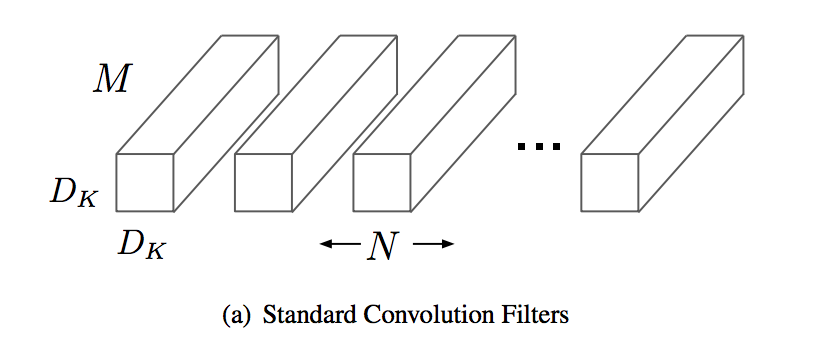
\includegraphics{assets/standard_conv.png}
\caption{Standard Convolution}
\end{figure}

\hypertarget{depthwise-convolution}{%
\paragraph{Depthwise Convolution}\label{depthwise-convolution}}

A depthwise convolution acts on each input channel separately with a
different kernel. \(M\) input channels implies there are \(M\)
\(D_k * D_k\) kernels. Also notice this results in \(N\) being set to 1.
If this doesn't make sense, think about the shape a kernel would have to
be to act upon an inidividual channel.

Computation cost:

\[
D_f * D_f * M * D_k * D_k
\]

\begin{figure}
\centering
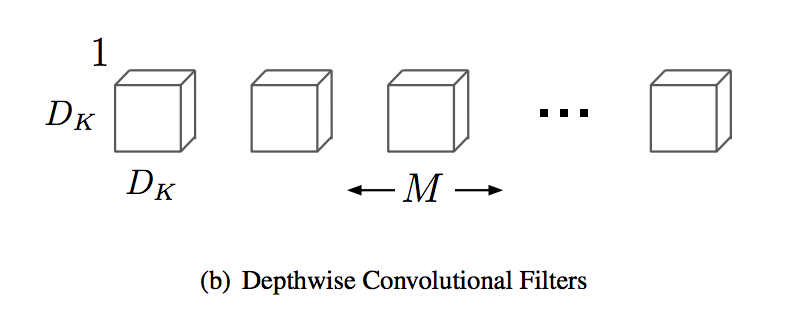
\includegraphics{assets/depthwise_conv.png}
\caption{Depthwise Convolution}
\end{figure}

\hypertarget{pointwise-convolution}{%
\paragraph{Pointwise Convolution}\label{pointwise-convolution}}

A pointwise convolution performs a 1x1 convolution, it's the same as a
vanilla convolution except the kernel size is \(1 * 1\).

Computation cost:

\[
D_k * D_k * D_f * D_f * M * N =
1 * 1 * D_f * D_f * M * N =
D_f * D_f * M * N
\]

\begin{figure}
\centering
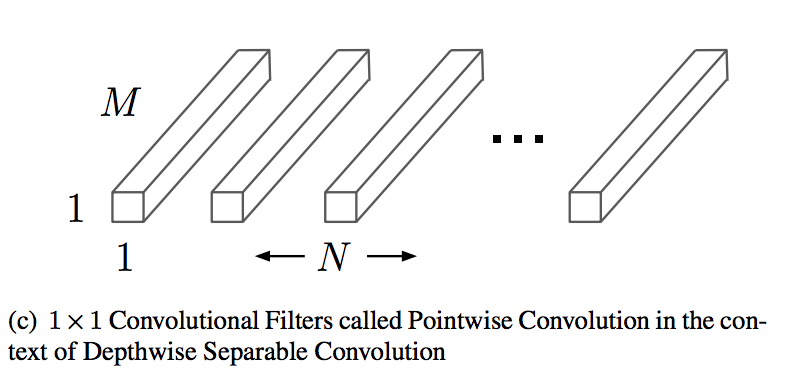
\includegraphics{assets/pointwise_conv.png}
\caption{Pointwise Convolution}
\end{figure}

Thus the total computation cost is for separable depthwise convolution:

\[
D_f * D_f * M * D_k * D_k + D_f * D_f * M * N
\]

which results in \(\frac{1}{N} + \frac{1}{D_k^2}\) reduction in
computation:

\[
\frac {D_f * D_f * M * D_k * D_k + D_f * D_f * M * N} {D_f * D_f * M * N * D_k * D_k} = 
\frac {D_k^2 + N} {D_k^2*N} = 
\frac {1}{N} + \frac{1}{D_k^2}
\]

\emph{MobileNets} use a 3x3 kernel, so assuming a large enough \(N\),
separable depthwise convnets are \textasciitilde{}9x more
computationally efficient than vanilla convolutions!

    \hypertarget{width-multiplier}{%
\subsubsection{Width Multiplier}\label{width-multiplier}}

The 2nd technique for reducing the computational cost is the ``width
multiplier'' which is a hyperparameter inhabiting the range {[}0, 1{]}
denoted here as \(\alpha\). \(\alpha\) reduces the number of input and
output channels proportionally:

\[
D_f * D_f * \alpha M * D_k * D_k + D_f * D_f * \alpha M * \alpha N
\]

    \hypertarget{resolution-multiplier}{%
\subsubsection{Resolution Multiplier}\label{resolution-multiplier}}

The 3rd technique for reducing the computational cost is the
``resolution multiplier'' which is a hyperparameter inhabiting the range
{[}0, 1{]} denoted here as \(\rho\). \(\rho\) reduces the size of the
input feature map:

\[
\rho D_f * \rho D_f * M * D_k * D_k + \rho D_f * \rho D_f * M * N
\]

    Combining the width and resolution multipliers results in a
computational cost of:

\[
\rho D_f * \rho D_f * a M * D_k * D_k + \rho D_f * \rho D_f * a M * a N
\]

Training \emph{MobileNets} with different values of \(\alpha\) and
\(\rho\) will result in different speed vs.~accuracy tradeoffs. The
folks at Google have run these experiments, the result are shown in the
graphic below:

\begin{figure}
\centering
\includegraphics{https://github.com/tensorflow/models/raw/master/research/slim/nets/mobilenet_v1.png}
\caption{MobileNets Graphic}
\end{figure}

    MACs (M) represents the number of multiplication-add operations in the
millions.

    \hypertarget{exercise-1---implement-separable-depthwise-convolution}{%
\subsubsection{Exercise 1 - Implement Separable Depthwise
Convolution}\label{exercise-1---implement-separable-depthwise-convolution}}

In this exercise you'll implement a separable depthwise convolution
block and compare the number of parameters to a standard convolution
block. For this exercise we'll assume the width and resolution
multipliers are set to 1.

Docs:

\begin{itemize}
\tightlist
\item
  \href{https://www.tensorflow.org/api_docs/python/tf/nn/depthwise_conv2d}{depthwise
  convolution}
\end{itemize}

    \begin{Verbatim}[commandchars=\\\{\}]
{\color{incolor}In [{\color{incolor}22}]:} \PY{k}{def} \PY{n+nf}{vanilla\PYZus{}conv\PYZus{}block}\PY{p}{(}\PY{n}{x}\PY{p}{,} \PY{n}{kernel\PYZus{}size}\PY{p}{,} \PY{n}{output\PYZus{}channels}\PY{p}{)}\PY{p}{:}
             \PY{l+s+sd}{\PYZdq{}\PYZdq{}\PYZdq{}}
         \PY{l+s+sd}{    Vanilla Conv \PYZhy{}\PYZgt{} Batch Norm \PYZhy{}\PYZgt{} ReLU}
         \PY{l+s+sd}{    \PYZdq{}\PYZdq{}\PYZdq{}}
             \PY{n}{x} \PY{o}{=} \PY{n}{tf}\PY{o}{.}\PY{n}{layers}\PY{o}{.}\PY{n}{conv2d}\PY{p}{(}
                 \PY{n}{x}\PY{p}{,} \PY{n}{output\PYZus{}channels}\PY{p}{,} \PY{n}{kernel\PYZus{}size}\PY{p}{,} \PY{p}{(}\PY{l+m+mi}{2}\PY{p}{,} \PY{l+m+mi}{2}\PY{p}{)}\PY{p}{,} \PY{n}{padding}\PY{o}{=}\PY{l+s+s1}{\PYZsq{}}\PY{l+s+s1}{SAME}\PY{l+s+s1}{\PYZsq{}}\PY{p}{)}
             \PY{n}{x} \PY{o}{=} \PY{n}{tf}\PY{o}{.}\PY{n}{layers}\PY{o}{.}\PY{n}{batch\PYZus{}normalization}\PY{p}{(}\PY{n}{x}\PY{p}{)}
             \PY{k}{return} \PY{n}{tf}\PY{o}{.}\PY{n}{nn}\PY{o}{.}\PY{n}{relu}\PY{p}{(}\PY{n}{x}\PY{p}{)}
         
         \PY{c+c1}{\PYZsh{} TODO: implement MobileNet conv block}
         \PY{k}{def} \PY{n+nf}{mobilenet\PYZus{}conv\PYZus{}block}\PY{p}{(}\PY{n}{x}\PY{p}{,} \PY{n}{kernel\PYZus{}size}\PY{p}{,} \PY{n}{output\PYZus{}channels}\PY{p}{)}\PY{p}{:}
             \PY{l+s+sd}{\PYZdq{}\PYZdq{}\PYZdq{}}
         \PY{l+s+sd}{    Depthwise Conv \PYZhy{}\PYZgt{} Batch Norm \PYZhy{}\PYZgt{} ReLU \PYZhy{}\PYZgt{} Pointwise Conv \PYZhy{}\PYZgt{} Batch Norm \PYZhy{}\PYZgt{} ReLU}
         \PY{l+s+sd}{    \PYZdq{}\PYZdq{}\PYZdq{}}
             \PY{n}{x} \PY{o}{=} \PY{n}{tf}\PY{o}{.}\PY{n}{nn}\PY{o}{.}\PY{n}{depthwise\PYZus{}conv2d}\PY{p}{(}
                 \PY{n}{x}\PY{p}{,} \PY{n}{tf}\PY{o}{.}\PY{n}{truncated\PYZus{}normal}\PY{p}{(}\PY{p}{(}\PY{n}{kernel\PYZus{}size}\PY{p}{,} \PY{n}{kernel\PYZus{}size}\PY{p}{,} \PY{n}{x}\PY{o}{.}\PY{n}{get\PYZus{}shape}\PY{p}{(}\PY{p}{)}\PY{o}{.}\PY{n}{as\PYZus{}list}\PY{p}{(}\PY{p}{)}\PY{p}{[}\PY{o}{\PYZhy{}}\PY{l+m+mi}{1}\PY{p}{]} \PY{p}{,} \PY{l+m+mi}{1}\PY{p}{)}\PY{p}{)}\PY{p}{,} 
                 \PY{p}{(}\PY{l+m+mi}{1}\PY{p}{,} \PY{l+m+mi}{2}\PY{p}{,} \PY{l+m+mi}{2}\PY{p}{,} \PY{l+m+mi}{1}\PY{p}{)}\PY{p}{,} \PY{n}{padding}\PY{o}{=}\PY{l+s+s1}{\PYZsq{}}\PY{l+s+s1}{SAME}\PY{l+s+s1}{\PYZsq{}}\PY{p}{)}
             \PY{n}{x} \PY{o}{=} \PY{n}{tf}\PY{o}{.}\PY{n}{layers}\PY{o}{.}\PY{n}{batch\PYZus{}normalization}\PY{p}{(}\PY{n}{x}\PY{p}{)}
             \PY{n}{x} \PY{o}{=} \PY{n}{tf}\PY{o}{.}\PY{n}{nn}\PY{o}{.}\PY{n}{relu}\PY{p}{(}\PY{n}{x}\PY{p}{)}
             
             \PY{n}{x} \PY{o}{=} \PY{n}{tf}\PY{o}{.}\PY{n}{layers}\PY{o}{.}\PY{n}{conv2d}\PY{p}{(}
                 \PY{n}{x}\PY{p}{,} \PY{n}{output\PYZus{}channels}\PY{p}{,} \PY{l+m+mi}{1}\PY{p}{,} \PY{p}{(}\PY{l+m+mi}{1}\PY{p}{,} \PY{l+m+mi}{1}\PY{p}{)}\PY{p}{,} \PY{n}{padding}\PY{o}{=}\PY{l+s+s1}{\PYZsq{}}\PY{l+s+s1}{SAME}\PY{l+s+s1}{\PYZsq{}}\PY{p}{)}
             \PY{n}{x} \PY{o}{=} \PY{n}{tf}\PY{o}{.}\PY{n}{layers}\PY{o}{.}\PY{n}{batch\PYZus{}normalization}\PY{p}{(}\PY{n}{x}\PY{p}{)}
             \PY{k}{return} \PY{n}{tf}\PY{o}{.}\PY{n}{nn}\PY{o}{.}\PY{n}{relu}\PY{p}{(}\PY{n}{x}\PY{p}{)}
\end{Verbatim}


    \textbf{\href{./exercise-solutions/e1.py}{Sample solution}}

Let's compare the number of parameters in each block.

    \begin{Verbatim}[commandchars=\\\{\}]
{\color{incolor}In [{\color{incolor}23}]:} \PY{c+c1}{\PYZsh{} constants but you can change them so I guess they\PYZsq{}re not so constant :)}
         \PY{n}{INPUT\PYZus{}CHANNELS} \PY{o}{=} \PY{l+m+mi}{32}
         \PY{n}{OUTPUT\PYZus{}CHANNELS} \PY{o}{=} \PY{l+m+mi}{512}
         \PY{n}{KERNEL\PYZus{}SIZE} \PY{o}{=} \PY{l+m+mi}{3}
         \PY{n}{IMG\PYZus{}HEIGHT} \PY{o}{=} \PY{l+m+mi}{256}
         \PY{n}{IMG\PYZus{}WIDTH} \PY{o}{=} \PY{l+m+mi}{256}
         
         \PY{k}{with} \PY{n}{tf}\PY{o}{.}\PY{n}{Session}\PY{p}{(}\PY{n}{graph}\PY{o}{=}\PY{n}{tf}\PY{o}{.}\PY{n}{Graph}\PY{p}{(}\PY{p}{)}\PY{p}{)} \PY{k}{as} \PY{n}{sess}\PY{p}{:}
             \PY{c+c1}{\PYZsh{} input}
             \PY{n}{x} \PY{o}{=} \PY{n}{tf}\PY{o}{.}\PY{n}{constant}\PY{p}{(}\PY{n}{np}\PY{o}{.}\PY{n}{random}\PY{o}{.}\PY{n}{randn}\PY{p}{(}\PY{l+m+mi}{1}\PY{p}{,} \PY{n}{IMG\PYZus{}HEIGHT}\PY{p}{,} \PY{n}{IMG\PYZus{}WIDTH}\PY{p}{,} \PY{n}{INPUT\PYZus{}CHANNELS}\PY{p}{)}\PY{p}{,} \PY{n}{dtype}\PY{o}{=}\PY{n}{tf}\PY{o}{.}\PY{n}{float32}\PY{p}{)}
         
             \PY{k}{with} \PY{n}{tf}\PY{o}{.}\PY{n}{variable\PYZus{}scope}\PY{p}{(}\PY{l+s+s1}{\PYZsq{}}\PY{l+s+s1}{vanilla}\PY{l+s+s1}{\PYZsq{}}\PY{p}{)}\PY{p}{:}
                 \PY{n}{vanilla\PYZus{}conv} \PY{o}{=} \PY{n}{vanilla\PYZus{}conv\PYZus{}block}\PY{p}{(}\PY{n}{x}\PY{p}{,} \PY{n}{KERNEL\PYZus{}SIZE}\PY{p}{,} \PY{n}{OUTPUT\PYZus{}CHANNELS}\PY{p}{)}
             \PY{k}{with} \PY{n}{tf}\PY{o}{.}\PY{n}{variable\PYZus{}scope}\PY{p}{(}\PY{l+s+s1}{\PYZsq{}}\PY{l+s+s1}{mobile}\PY{l+s+s1}{\PYZsq{}}\PY{p}{)}\PY{p}{:}
                 \PY{n}{mobilenet\PYZus{}conv} \PY{o}{=} \PY{n}{mobilenet\PYZus{}conv\PYZus{}block}\PY{p}{(}\PY{n}{x}\PY{p}{,} \PY{n}{KERNEL\PYZus{}SIZE}\PY{p}{,} \PY{n}{OUTPUT\PYZus{}CHANNELS}\PY{p}{)}
         
             \PY{n}{vanilla\PYZus{}params} \PY{o}{=} \PY{p}{[}
                 \PY{p}{(}\PY{n}{v}\PY{o}{.}\PY{n}{name}\PY{p}{,} \PY{n}{np}\PY{o}{.}\PY{n}{prod}\PY{p}{(}\PY{n}{v}\PY{o}{.}\PY{n}{get\PYZus{}shape}\PY{p}{(}\PY{p}{)}\PY{o}{.}\PY{n}{as\PYZus{}list}\PY{p}{(}\PY{p}{)}\PY{p}{)}\PY{p}{)}
                 \PY{k}{for} \PY{n}{v} \PY{o+ow}{in} \PY{n}{tf}\PY{o}{.}\PY{n}{get\PYZus{}collection}\PY{p}{(}\PY{n}{tf}\PY{o}{.}\PY{n}{GraphKeys}\PY{o}{.}\PY{n}{TRAINABLE\PYZus{}VARIABLES}\PY{p}{,} \PY{l+s+s1}{\PYZsq{}}\PY{l+s+s1}{vanilla}\PY{l+s+s1}{\PYZsq{}}\PY{p}{)}
             \PY{p}{]}
             \PY{n}{mobile\PYZus{}params} \PY{o}{=} \PY{p}{[}
                 \PY{p}{(}\PY{n}{v}\PY{o}{.}\PY{n}{name}\PY{p}{,} \PY{n}{np}\PY{o}{.}\PY{n}{prod}\PY{p}{(}\PY{n}{v}\PY{o}{.}\PY{n}{get\PYZus{}shape}\PY{p}{(}\PY{p}{)}\PY{o}{.}\PY{n}{as\PYZus{}list}\PY{p}{(}\PY{p}{)}\PY{p}{)}\PY{p}{)}
                 \PY{k}{for} \PY{n}{v} \PY{o+ow}{in} \PY{n}{tf}\PY{o}{.}\PY{n}{get\PYZus{}collection}\PY{p}{(}\PY{n}{tf}\PY{o}{.}\PY{n}{GraphKeys}\PY{o}{.}\PY{n}{TRAINABLE\PYZus{}VARIABLES}\PY{p}{,} \PY{l+s+s1}{\PYZsq{}}\PY{l+s+s1}{mobile}\PY{l+s+s1}{\PYZsq{}}\PY{p}{)}
             \PY{p}{]}
         
             \PY{n+nb}{print}\PY{p}{(}\PY{l+s+s2}{\PYZdq{}}\PY{l+s+s2}{VANILLA CONV BLOCK}\PY{l+s+s2}{\PYZdq{}}\PY{p}{)}
             \PY{n}{total\PYZus{}vanilla\PYZus{}params} \PY{o}{=} \PY{n+nb}{sum}\PY{p}{(}\PY{p}{[}\PY{n}{p}\PY{p}{[}\PY{l+m+mi}{1}\PY{p}{]} \PY{k}{for} \PY{n}{p} \PY{o+ow}{in} \PY{n}{vanilla\PYZus{}params}\PY{p}{]}\PY{p}{)}
             \PY{k}{for} \PY{n}{p} \PY{o+ow}{in} \PY{n}{vanilla\PYZus{}params}\PY{p}{:}
                 \PY{n+nb}{print}\PY{p}{(}\PY{l+s+s2}{\PYZdq{}}\PY{l+s+s2}{Variable }\PY{l+s+si}{\PYZob{}0\PYZcb{}}\PY{l+s+s2}{: number of params = }\PY{l+s+si}{\PYZob{}1\PYZcb{}}\PY{l+s+s2}{\PYZdq{}}\PY{o}{.}\PY{n}{format}\PY{p}{(}\PY{n}{p}\PY{p}{[}\PY{l+m+mi}{0}\PY{p}{]}\PY{p}{,} \PY{n}{p}\PY{p}{[}\PY{l+m+mi}{1}\PY{p}{]}\PY{p}{)}\PY{p}{)}
             \PY{n+nb}{print}\PY{p}{(}\PY{l+s+s2}{\PYZdq{}}\PY{l+s+s2}{Total number of params =}\PY{l+s+s2}{\PYZdq{}}\PY{p}{,} \PY{n}{total\PYZus{}vanilla\PYZus{}params}\PY{p}{)}
             \PY{n+nb}{print}\PY{p}{(}\PY{p}{)}
         
             \PY{n+nb}{print}\PY{p}{(}\PY{l+s+s2}{\PYZdq{}}\PY{l+s+s2}{MOBILENET CONV BLOCK}\PY{l+s+s2}{\PYZdq{}}\PY{p}{)}
             \PY{n}{total\PYZus{}mobile\PYZus{}params} \PY{o}{=} \PY{n+nb}{sum}\PY{p}{(}\PY{p}{[}\PY{n}{p}\PY{p}{[}\PY{l+m+mi}{1}\PY{p}{]} \PY{k}{for} \PY{n}{p} \PY{o+ow}{in} \PY{n}{mobile\PYZus{}params}\PY{p}{]}\PY{p}{)}
             \PY{k}{for} \PY{n}{p} \PY{o+ow}{in} \PY{n}{mobile\PYZus{}params}\PY{p}{:}
                 \PY{n+nb}{print}\PY{p}{(}\PY{l+s+s2}{\PYZdq{}}\PY{l+s+s2}{Variable }\PY{l+s+si}{\PYZob{}0\PYZcb{}}\PY{l+s+s2}{: number of params = }\PY{l+s+si}{\PYZob{}1\PYZcb{}}\PY{l+s+s2}{\PYZdq{}}\PY{o}{.}\PY{n}{format}\PY{p}{(}\PY{n}{p}\PY{p}{[}\PY{l+m+mi}{0}\PY{p}{]}\PY{p}{,} \PY{n}{p}\PY{p}{[}\PY{l+m+mi}{1}\PY{p}{]}\PY{p}{)}\PY{p}{)}
             \PY{n+nb}{print}\PY{p}{(}\PY{l+s+s2}{\PYZdq{}}\PY{l+s+s2}{Total number of params =}\PY{l+s+s2}{\PYZdq{}}\PY{p}{,} \PY{n}{total\PYZus{}mobile\PYZus{}params}\PY{p}{)}
             \PY{n+nb}{print}\PY{p}{(}\PY{p}{)}
         
             \PY{n+nb}{print}\PY{p}{(}\PY{l+s+s2}{\PYZdq{}}\PY{l+s+si}{\PYZob{}0:.3f\PYZcb{}}\PY{l+s+s2}{x parameter reduction}\PY{l+s+s2}{\PYZdq{}}\PY{o}{.}\PY{n}{format}\PY{p}{(}\PY{n}{total\PYZus{}vanilla\PYZus{}params} \PY{o}{/}
                                                      \PY{n}{total\PYZus{}mobile\PYZus{}params}\PY{p}{)}\PY{p}{)}
\end{Verbatim}


    \begin{Verbatim}[commandchars=\\\{\}]
VANILLA CONV BLOCK
Variable vanilla/conv2d/kernel:0: number of params = 147456
Variable vanilla/conv2d/bias:0: number of params = 512
Variable vanilla/batch\_normalization/gamma:0: number of params = 512
Variable vanilla/batch\_normalization/beta:0: number of params = 512
Total number of params = 148992

MOBILENET CONV BLOCK
Variable mobile/batch\_normalization/gamma:0: number of params = 32
Variable mobile/batch\_normalization/beta:0: number of params = 32
Variable mobile/conv2d/kernel:0: number of params = 16384
Variable mobile/conv2d/bias:0: number of params = 512
Variable mobile/batch\_normalization\_1/gamma:0: number of params = 512
Variable mobile/batch\_normalization\_1/beta:0: number of params = 512
Total number of params = 17984

8.285x parameter reduction

    \end{Verbatim}

    Your solution should show the majority of the parameters in
\emph{MobileNet} block stem from the pointwise convolution.

    \hypertarget{mobilenet-ssd}{%
\subsection{\texorpdfstring{\emph{MobileNet}
SSD}{MobileNet SSD}}\label{mobilenet-ssd}}

In this section you'll use a pretrained \emph{MobileNet}
\href{https://arxiv.org/abs/1512.02325}{SSD} model to perform object
detection. You can download the \emph{MobileNet} SSD and other models
from the
\href{https://github.com/tensorflow/models/blob/master/research/object_detection/g3doc/detection_model_zoo.md}{TensorFlow
detection model zoo}. \href{https://arxiv.org/abs/1611.10012}{Paper}
describing comparing several object detection models.

Alright, let's get into SSD!

    \hypertarget{single-shot-detection-ssd}{%
\subsubsection{Single Shot Detection
(SSD)}\label{single-shot-detection-ssd}}

Many previous works in object detection involve more than one training
phase. For example, the
\href{https://arxiv.org/abs/1506.01497}{Faster-RCNN} architecture first
trains a Region Proposal Network (RPN) which decides which regions of
the image are worth drawing a box around. RPN is then merged with a
pretrained model for classification (classifies the regions). The image
below is an RPN:

\begin{figure}
\centering
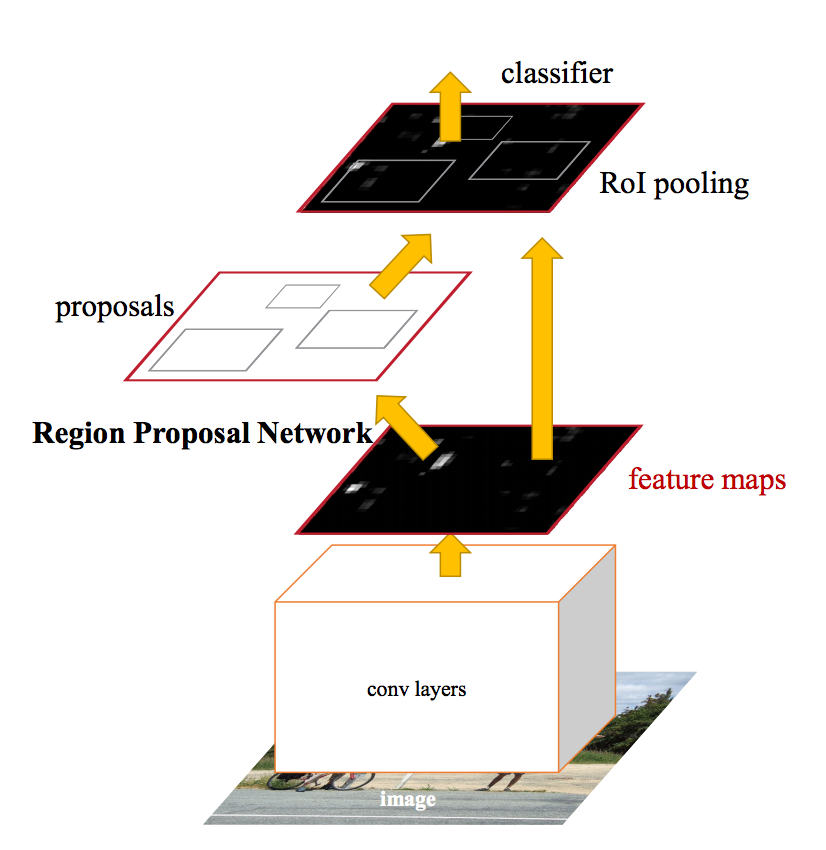
\includegraphics{./assets/faster-rcnn.png}
\caption{Faster-RCNN Visual}
\end{figure}

    The SSD architecture is a single convolutional network which learns to
predict bounding box locations and classify the locations in one pass.
Put differently, SSD can be trained end to end while Faster-RCNN cannot.
The SSD architecture consists of a base network followed by several
convolutional layers:

\begin{figure}
\centering
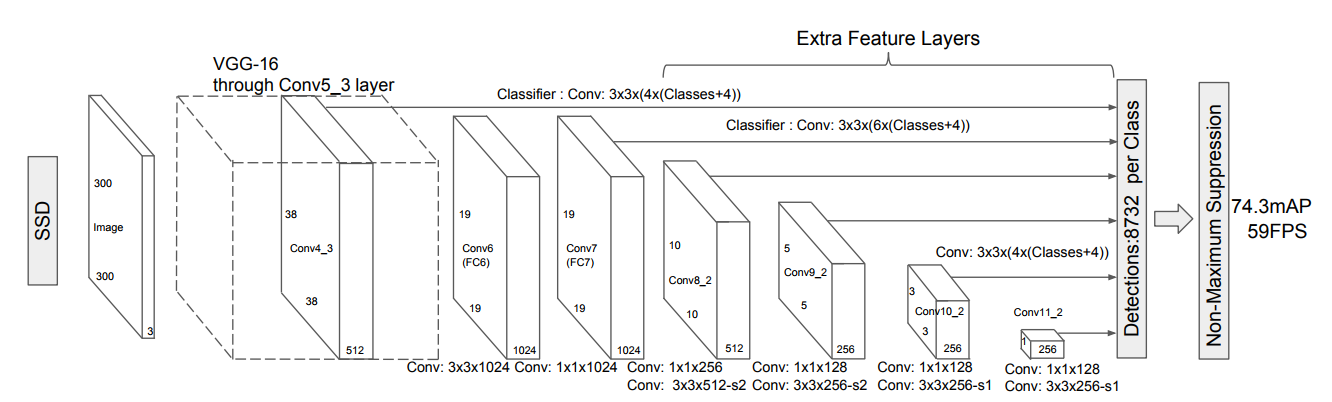
\includegraphics{./assets/ssd_architecture.png}
\caption{SSD Visual}
\end{figure}

\textbf{NOTE:} In this lab the base network is a MobileNet (instead of
VGG16.)

\hypertarget{detecting-boxes}{%
\paragraph{Detecting Boxes}\label{detecting-boxes}}

SSD operates on feature maps to predict bounding box locations. Recall a
feature map is of size \(D_f * D_f * M\). For each feature map location
\(k\) bounding boxes are predicted. Each bounding box carries with it
the following information:

\begin{itemize}
\tightlist
\item
  4 corner bounding box \textbf{offset} locations \((cx, cy, w, h)\)
\item
  \(C\) class probabilities \((c_1, c_2, ..., c_p)\)
\end{itemize}

SSD \textbf{does not} predict the shape of the box, rather just where
the box is. The \(k\) bounding boxes each have a predetermined shape.
This is illustrated in the figure below:

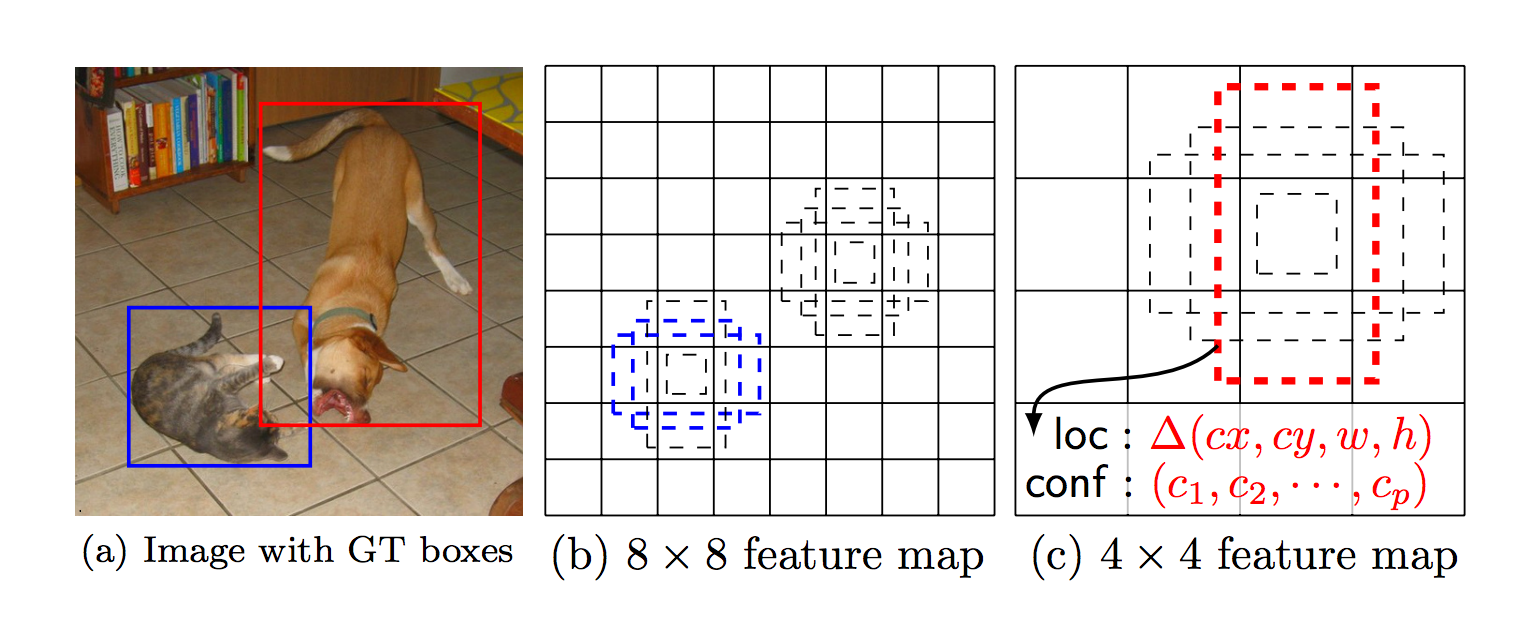
\includegraphics{./assets/ssd_feature_maps.png}

The shapes are set prior to actual training. For example, In figure (c)
in the above picture there are 4 boxes, meaning \(k\) = 4.

    \hypertarget{exercise-2---ssd-feature-maps}{%
\subsubsection{Exercise 2 - SSD Feature
Maps}\label{exercise-2---ssd-feature-maps}}

It would be a good exercise to read the SSD paper prior to a answering
the following questions.

\textbf{\emph{Q: Why does SSD use several differently sized feature maps
to predict detections?}}

    A: Your answer here

\textbf{\href{./exercise-solutions/e2.md}{Sample answer}}

    The current approach leaves us with thousands of bounding box
candidates, clearly the vast majority of them are nonsensical.

\hypertarget{exercise-3---filtering-bounding-boxes}{%
\subsubsection{Exercise 3 - Filtering Bounding
Boxes}\label{exercise-3---filtering-bounding-boxes}}

\textbf{\emph{Q: What are some ways which we can filter nonsensical
bounding boxes?}}

    A: Your answer here

\textbf{\href{./exercise-solutions/e3.md}{Sample answer}}

    \hypertarget{loss}{%
\paragraph{Loss}\label{loss}}

With the final set of matched boxes we can compute the loss:

\[
L = \frac {1} {N} * ( L_{class} + L_{box})
\]

where \(N\) is the total number of matched boxes, \(L_{class}\) is a
softmax loss for classification, and \(L_{box}\) is a L1 smooth loss
representing the error of the matched boxes with the ground truth boxes.
L1 smooth loss is a modification of L1 loss which is more robust to
outliers. In the event \(N\) is 0 the loss is set 0.

    \hypertarget{ssd-summary}{%
\subsubsection{SSD Summary}\label{ssd-summary}}

\begin{itemize}
\tightlist
\item
  Starts from a base model pretrained on ImageNet.
\item
  The base model is extended by several convolutional layers.
\item
  Each feature map is used to predict bounding boxes. Diversity in
  feature map size allows object detection at different resolutions.
\item
  Boxes are filtered by IoU metrics and hard negative mining.
\item
  Loss is a combination of classification (softmax) and dectection
  (smooth L1)
\item
  Model can be trained end to end.
\end{itemize}

    \hypertarget{object-detection-inference}{%
\subsection{Object Detection
Inference}\label{object-detection-inference}}

In this part of the lab you'll detect objects using pretrained object
detection models. You can download the pretrained models from the
\href{https://github.com/tensorflow/models/blob/master/research/object_detection/g3doc/detection_model_zoo.md}{model
zoo}.

    \begin{Verbatim}[commandchars=\\\{\}]
{\color{incolor}In [{\color{incolor}27}]:} \PY{c+c1}{\PYZsh{} Frozen inference graph files. NOTE: change the path to where you saved the models.}
         \PY{n}{SSD\PYZus{}GRAPH\PYZus{}FILE} \PY{o}{=} \PY{l+s+s1}{\PYZsq{}}\PY{l+s+s1}{ssd\PYZus{}mobilenet\PYZus{}v1\PYZus{}coco\PYZus{}2017\PYZus{}11\PYZus{}17/frozen\PYZus{}inference\PYZus{}graph.pb}\PY{l+s+s1}{\PYZsq{}}
         \PY{n}{RFCN\PYZus{}GRAPH\PYZus{}FILE} \PY{o}{=} \PY{l+s+s1}{\PYZsq{}}\PY{l+s+s1}{rfcn\PYZus{}resnet101\PYZus{}coco\PYZus{}2018\PYZus{}01\PYZus{}28/frozen\PYZus{}inference\PYZus{}graph.pb}\PY{l+s+s1}{\PYZsq{}}
         \PY{n}{FASTER\PYZus{}RCNN\PYZus{}GRAPH\PYZus{}FILE} \PY{o}{=} \PY{l+s+s1}{\PYZsq{}}\PY{l+s+s1}{faster\PYZus{}rcnn\PYZus{}inception\PYZus{}resnet\PYZus{}v2\PYZus{}atrous\PYZus{}coco\PYZus{}2018\PYZus{}01\PYZus{}28/frozen\PYZus{}inference\PYZus{}graph.pb}\PY{l+s+s1}{\PYZsq{}}
\end{Verbatim}


    Below are utility functions. The main purpose of these is to draw the
bounding boxes back onto the original image.

    \begin{Verbatim}[commandchars=\\\{\}]
{\color{incolor}In [{\color{incolor}28}]:} \PY{c+c1}{\PYZsh{} Colors (one for each class)}
         \PY{n}{cmap} \PY{o}{=} \PY{n}{ImageColor}\PY{o}{.}\PY{n}{colormap}
         \PY{n+nb}{print}\PY{p}{(}\PY{l+s+s2}{\PYZdq{}}\PY{l+s+s2}{Number of colors =}\PY{l+s+s2}{\PYZdq{}}\PY{p}{,} \PY{n+nb}{len}\PY{p}{(}\PY{n}{cmap}\PY{p}{)}\PY{p}{)}
         \PY{n}{COLOR\PYZus{}LIST} \PY{o}{=} \PY{n+nb}{sorted}\PY{p}{(}\PY{p}{[}\PY{n}{c} \PY{k}{for} \PY{n}{c} \PY{o+ow}{in} \PY{n}{cmap}\PY{o}{.}\PY{n}{keys}\PY{p}{(}\PY{p}{)}\PY{p}{]}\PY{p}{)}
         
         \PY{c+c1}{\PYZsh{}}
         \PY{c+c1}{\PYZsh{} Utility funcs}
         \PY{c+c1}{\PYZsh{}}
         
         \PY{k}{def} \PY{n+nf}{filter\PYZus{}boxes}\PY{p}{(}\PY{n}{min\PYZus{}score}\PY{p}{,} \PY{n}{boxes}\PY{p}{,} \PY{n}{scores}\PY{p}{,} \PY{n}{classes}\PY{p}{)}\PY{p}{:}
             \PY{l+s+sd}{\PYZdq{}\PYZdq{}\PYZdq{}Return boxes with a confidence \PYZgt{}= `min\PYZus{}score`\PYZdq{}\PYZdq{}\PYZdq{}}
             \PY{n}{n} \PY{o}{=} \PY{n+nb}{len}\PY{p}{(}\PY{n}{classes}\PY{p}{)}
             \PY{n}{idxs} \PY{o}{=} \PY{p}{[}\PY{p}{]}
             \PY{k}{for} \PY{n}{i} \PY{o+ow}{in} \PY{n+nb}{range}\PY{p}{(}\PY{n}{n}\PY{p}{)}\PY{p}{:}
                 \PY{k}{if} \PY{n}{scores}\PY{p}{[}\PY{n}{i}\PY{p}{]} \PY{o}{\PYZgt{}}\PY{o}{=} \PY{n}{min\PYZus{}score}\PY{p}{:}
                     \PY{n}{idxs}\PY{o}{.}\PY{n}{append}\PY{p}{(}\PY{n}{i}\PY{p}{)}
             
             \PY{n}{filtered\PYZus{}boxes} \PY{o}{=} \PY{n}{boxes}\PY{p}{[}\PY{n}{idxs}\PY{p}{,} \PY{o}{.}\PY{o}{.}\PY{o}{.}\PY{p}{]}
             \PY{n}{filtered\PYZus{}scores} \PY{o}{=} \PY{n}{scores}\PY{p}{[}\PY{n}{idxs}\PY{p}{,} \PY{o}{.}\PY{o}{.}\PY{o}{.}\PY{p}{]}
             \PY{n}{filtered\PYZus{}classes} \PY{o}{=} \PY{n}{classes}\PY{p}{[}\PY{n}{idxs}\PY{p}{,} \PY{o}{.}\PY{o}{.}\PY{o}{.}\PY{p}{]}
             \PY{k}{return} \PY{n}{filtered\PYZus{}boxes}\PY{p}{,} \PY{n}{filtered\PYZus{}scores}\PY{p}{,} \PY{n}{filtered\PYZus{}classes}
         
         \PY{k}{def} \PY{n+nf}{to\PYZus{}image\PYZus{}coords}\PY{p}{(}\PY{n}{boxes}\PY{p}{,} \PY{n}{height}\PY{p}{,} \PY{n}{width}\PY{p}{)}\PY{p}{:}
             \PY{l+s+sd}{\PYZdq{}\PYZdq{}\PYZdq{}}
         \PY{l+s+sd}{    The original box coordinate output is normalized, i.e [0, 1].}
         \PY{l+s+sd}{    }
         \PY{l+s+sd}{    This converts it back to the original coordinate based on the image}
         \PY{l+s+sd}{    size.}
         \PY{l+s+sd}{    \PYZdq{}\PYZdq{}\PYZdq{}}
             \PY{n}{box\PYZus{}coords} \PY{o}{=} \PY{n}{np}\PY{o}{.}\PY{n}{zeros\PYZus{}like}\PY{p}{(}\PY{n}{boxes}\PY{p}{)}
             \PY{n}{box\PYZus{}coords}\PY{p}{[}\PY{p}{:}\PY{p}{,} \PY{l+m+mi}{0}\PY{p}{]} \PY{o}{=} \PY{n}{boxes}\PY{p}{[}\PY{p}{:}\PY{p}{,} \PY{l+m+mi}{0}\PY{p}{]} \PY{o}{*} \PY{n}{height}
             \PY{n}{box\PYZus{}coords}\PY{p}{[}\PY{p}{:}\PY{p}{,} \PY{l+m+mi}{1}\PY{p}{]} \PY{o}{=} \PY{n}{boxes}\PY{p}{[}\PY{p}{:}\PY{p}{,} \PY{l+m+mi}{1}\PY{p}{]} \PY{o}{*} \PY{n}{width}
             \PY{n}{box\PYZus{}coords}\PY{p}{[}\PY{p}{:}\PY{p}{,} \PY{l+m+mi}{2}\PY{p}{]} \PY{o}{=} \PY{n}{boxes}\PY{p}{[}\PY{p}{:}\PY{p}{,} \PY{l+m+mi}{2}\PY{p}{]} \PY{o}{*} \PY{n}{height}
             \PY{n}{box\PYZus{}coords}\PY{p}{[}\PY{p}{:}\PY{p}{,} \PY{l+m+mi}{3}\PY{p}{]} \PY{o}{=} \PY{n}{boxes}\PY{p}{[}\PY{p}{:}\PY{p}{,} \PY{l+m+mi}{3}\PY{p}{]} \PY{o}{*} \PY{n}{width}
             
             \PY{k}{return} \PY{n}{box\PYZus{}coords}
         
         \PY{k}{def} \PY{n+nf}{draw\PYZus{}boxes}\PY{p}{(}\PY{n}{image}\PY{p}{,} \PY{n}{boxes}\PY{p}{,} \PY{n}{classes}\PY{p}{,} \PY{n}{thickness}\PY{o}{=}\PY{l+m+mi}{4}\PY{p}{)}\PY{p}{:}
             \PY{l+s+sd}{\PYZdq{}\PYZdq{}\PYZdq{}Draw bounding boxes on the image\PYZdq{}\PYZdq{}\PYZdq{}}
             \PY{n}{draw} \PY{o}{=} \PY{n}{ImageDraw}\PY{o}{.}\PY{n}{Draw}\PY{p}{(}\PY{n}{image}\PY{p}{)}
             \PY{k}{for} \PY{n}{i} \PY{o+ow}{in} \PY{n+nb}{range}\PY{p}{(}\PY{n+nb}{len}\PY{p}{(}\PY{n}{boxes}\PY{p}{)}\PY{p}{)}\PY{p}{:}
                 \PY{n}{bot}\PY{p}{,} \PY{n}{left}\PY{p}{,} \PY{n}{top}\PY{p}{,} \PY{n}{right} \PY{o}{=} \PY{n}{boxes}\PY{p}{[}\PY{n}{i}\PY{p}{,} \PY{o}{.}\PY{o}{.}\PY{o}{.}\PY{p}{]}
                 \PY{n}{class\PYZus{}id} \PY{o}{=} \PY{n+nb}{int}\PY{p}{(}\PY{n}{classes}\PY{p}{[}\PY{n}{i}\PY{p}{]}\PY{p}{)}
                 \PY{n}{color} \PY{o}{=} \PY{n}{COLOR\PYZus{}LIST}\PY{p}{[}\PY{n}{class\PYZus{}id}\PY{p}{]}
                 \PY{n}{draw}\PY{o}{.}\PY{n}{line}\PY{p}{(}\PY{p}{[}\PY{p}{(}\PY{n}{left}\PY{p}{,} \PY{n}{top}\PY{p}{)}\PY{p}{,} \PY{p}{(}\PY{n}{left}\PY{p}{,} \PY{n}{bot}\PY{p}{)}\PY{p}{,} \PY{p}{(}\PY{n}{right}\PY{p}{,} \PY{n}{bot}\PY{p}{)}\PY{p}{,} \PY{p}{(}\PY{n}{right}\PY{p}{,} \PY{n}{top}\PY{p}{)}\PY{p}{,} \PY{p}{(}\PY{n}{left}\PY{p}{,} \PY{n}{top}\PY{p}{)}\PY{p}{]}\PY{p}{,} \PY{n}{width}\PY{o}{=}\PY{n}{thickness}\PY{p}{,} \PY{n}{fill}\PY{o}{=}\PY{n}{color}\PY{p}{)}
                 
         \PY{k}{def} \PY{n+nf}{load\PYZus{}graph}\PY{p}{(}\PY{n}{graph\PYZus{}file}\PY{p}{)}\PY{p}{:}
             \PY{l+s+sd}{\PYZdq{}\PYZdq{}\PYZdq{}Loads a frozen inference graph\PYZdq{}\PYZdq{}\PYZdq{}}
             \PY{n}{graph} \PY{o}{=} \PY{n}{tf}\PY{o}{.}\PY{n}{Graph}\PY{p}{(}\PY{p}{)}
             \PY{k}{with} \PY{n}{graph}\PY{o}{.}\PY{n}{as\PYZus{}default}\PY{p}{(}\PY{p}{)}\PY{p}{:}
                 \PY{n}{od\PYZus{}graph\PYZus{}def} \PY{o}{=} \PY{n}{tf}\PY{o}{.}\PY{n}{GraphDef}\PY{p}{(}\PY{p}{)}
                 \PY{k}{with} \PY{n}{tf}\PY{o}{.}\PY{n}{gfile}\PY{o}{.}\PY{n}{GFile}\PY{p}{(}\PY{n}{graph\PYZus{}file}\PY{p}{,} \PY{l+s+s1}{\PYZsq{}}\PY{l+s+s1}{rb}\PY{l+s+s1}{\PYZsq{}}\PY{p}{)} \PY{k}{as} \PY{n}{fid}\PY{p}{:}
                     \PY{n}{serialized\PYZus{}graph} \PY{o}{=} \PY{n}{fid}\PY{o}{.}\PY{n}{read}\PY{p}{(}\PY{p}{)}
                     \PY{n}{od\PYZus{}graph\PYZus{}def}\PY{o}{.}\PY{n}{ParseFromString}\PY{p}{(}\PY{n}{serialized\PYZus{}graph}\PY{p}{)}
                     \PY{n}{tf}\PY{o}{.}\PY{n}{import\PYZus{}graph\PYZus{}def}\PY{p}{(}\PY{n}{od\PYZus{}graph\PYZus{}def}\PY{p}{,} \PY{n}{name}\PY{o}{=}\PY{l+s+s1}{\PYZsq{}}\PY{l+s+s1}{\PYZsq{}}\PY{p}{)}
             \PY{k}{return} \PY{n}{graph}
\end{Verbatim}


    \begin{Verbatim}[commandchars=\\\{\}]
Number of colors = 148

    \end{Verbatim}

    Below we load the graph and extract the relevant tensors using
\href{https://www.tensorflow.org/api_docs/python/tf/Graph\#get_tensor_by_name}{\texttt{get\_tensor\_by\_name}}.
These tensors reflect the input and outputs of the graph, or least the
ones we care about for detecting objects.

    \begin{Verbatim}[commandchars=\\\{\}]
{\color{incolor}In [{\color{incolor}30}]:} \PY{n}{detection\PYZus{}graph} \PY{o}{=} \PY{n}{load\PYZus{}graph}\PY{p}{(}\PY{n}{SSD\PYZus{}GRAPH\PYZus{}FILE}\PY{p}{)}
         \PY{c+c1}{\PYZsh{} detection\PYZus{}graph = load\PYZus{}graph(RFCN\PYZus{}GRAPH\PYZus{}FILE)}
         \PY{c+c1}{\PYZsh{} detection\PYZus{}graph = load\PYZus{}graph(FASTER\PYZus{}RCNN\PYZus{}GRAPH\PYZus{}FILE)}
         
         \PY{c+c1}{\PYZsh{} The input placeholder for the image.}
         \PY{c+c1}{\PYZsh{} `get\PYZus{}tensor\PYZus{}by\PYZus{}name` returns the Tensor with the associated name in the Graph.}
         \PY{n}{image\PYZus{}tensor} \PY{o}{=} \PY{n}{detection\PYZus{}graph}\PY{o}{.}\PY{n}{get\PYZus{}tensor\PYZus{}by\PYZus{}name}\PY{p}{(}\PY{l+s+s1}{\PYZsq{}}\PY{l+s+s1}{image\PYZus{}tensor:0}\PY{l+s+s1}{\PYZsq{}}\PY{p}{)}
         
         \PY{c+c1}{\PYZsh{} Each box represents a part of the image where a particular object was detected.}
         \PY{n}{detection\PYZus{}boxes} \PY{o}{=} \PY{n}{detection\PYZus{}graph}\PY{o}{.}\PY{n}{get\PYZus{}tensor\PYZus{}by\PYZus{}name}\PY{p}{(}\PY{l+s+s1}{\PYZsq{}}\PY{l+s+s1}{detection\PYZus{}boxes:0}\PY{l+s+s1}{\PYZsq{}}\PY{p}{)}
         
         \PY{c+c1}{\PYZsh{} Each score represent how level of confidence for each of the objects.}
         \PY{c+c1}{\PYZsh{} Score is shown on the result image, together with the class label.}
         \PY{n}{detection\PYZus{}scores} \PY{o}{=} \PY{n}{detection\PYZus{}graph}\PY{o}{.}\PY{n}{get\PYZus{}tensor\PYZus{}by\PYZus{}name}\PY{p}{(}\PY{l+s+s1}{\PYZsq{}}\PY{l+s+s1}{detection\PYZus{}scores:0}\PY{l+s+s1}{\PYZsq{}}\PY{p}{)}
         
         \PY{c+c1}{\PYZsh{} The classification of the object (integer id).}
         \PY{n}{detection\PYZus{}classes} \PY{o}{=} \PY{n}{detection\PYZus{}graph}\PY{o}{.}\PY{n}{get\PYZus{}tensor\PYZus{}by\PYZus{}name}\PY{p}{(}\PY{l+s+s1}{\PYZsq{}}\PY{l+s+s1}{detection\PYZus{}classes:0}\PY{l+s+s1}{\PYZsq{}}\PY{p}{)}
\end{Verbatim}


    Run detection and classification on a sample image.

    \begin{Verbatim}[commandchars=\\\{\}]
{\color{incolor}In [{\color{incolor}36}]:} \PY{c+c1}{\PYZsh{} Load a sample image.}
         \PY{n}{image} \PY{o}{=} \PY{n}{Image}\PY{o}{.}\PY{n}{open}\PY{p}{(}\PY{l+s+s1}{\PYZsq{}}\PY{l+s+s1}{./assets/sample1.jpg}\PY{l+s+s1}{\PYZsq{}}\PY{p}{)}
         \PY{n}{image\PYZus{}np} \PY{o}{=} \PY{n}{np}\PY{o}{.}\PY{n}{expand\PYZus{}dims}\PY{p}{(}\PY{n}{np}\PY{o}{.}\PY{n}{asarray}\PY{p}{(}\PY{n}{image}\PY{p}{,} \PY{n}{dtype}\PY{o}{=}\PY{n}{np}\PY{o}{.}\PY{n}{uint8}\PY{p}{)}\PY{p}{,} \PY{l+m+mi}{0}\PY{p}{)}
         
         \PY{k}{with} \PY{n}{tf}\PY{o}{.}\PY{n}{Session}\PY{p}{(}\PY{n}{graph}\PY{o}{=}\PY{n}{detection\PYZus{}graph}\PY{p}{)} \PY{k}{as} \PY{n}{sess}\PY{p}{:}                
             \PY{c+c1}{\PYZsh{} Actual detection.}
             \PY{p}{(}\PY{n}{boxes}\PY{p}{,} \PY{n}{scores}\PY{p}{,} \PY{n}{classes}\PY{p}{)} \PY{o}{=} \PY{n}{sess}\PY{o}{.}\PY{n}{run}\PY{p}{(}\PY{p}{[}\PY{n}{detection\PYZus{}boxes}\PY{p}{,} \PY{n}{detection\PYZus{}scores}\PY{p}{,} \PY{n}{detection\PYZus{}classes}\PY{p}{]}\PY{p}{,} 
                                                 \PY{n}{feed\PYZus{}dict}\PY{o}{=}\PY{p}{\PYZob{}}\PY{n}{image\PYZus{}tensor}\PY{p}{:} \PY{n}{image\PYZus{}np}\PY{p}{\PYZcb{}}\PY{p}{)}
         
             \PY{c+c1}{\PYZsh{} Remove unnecessary dimensions}
             \PY{n}{boxes} \PY{o}{=} \PY{n}{np}\PY{o}{.}\PY{n}{squeeze}\PY{p}{(}\PY{n}{boxes}\PY{p}{)}
             \PY{n}{scores} \PY{o}{=} \PY{n}{np}\PY{o}{.}\PY{n}{squeeze}\PY{p}{(}\PY{n}{scores}\PY{p}{)}
             \PY{n}{classes} \PY{o}{=} \PY{n}{np}\PY{o}{.}\PY{n}{squeeze}\PY{p}{(}\PY{n}{classes}\PY{p}{)}
         
             \PY{n}{confidence\PYZus{}cutoff} \PY{o}{=} \PY{l+m+mf}{0.8}
             \PY{c+c1}{\PYZsh{} Filter boxes with a confidence score less than `confidence\PYZus{}cutoff`}
             \PY{n}{boxes}\PY{p}{,} \PY{n}{scores}\PY{p}{,} \PY{n}{classes} \PY{o}{=} \PY{n}{filter\PYZus{}boxes}\PY{p}{(}\PY{n}{confidence\PYZus{}cutoff}\PY{p}{,} \PY{n}{boxes}\PY{p}{,} \PY{n}{scores}\PY{p}{,} \PY{n}{classes}\PY{p}{)}
             \PY{n+nb}{print}\PY{p}{(}\PY{n}{boxes}\PY{p}{)}
             \PY{n+nb}{print}\PY{p}{(}\PY{n}{scores}\PY{p}{)}
             \PY{n+nb}{print}\PY{p}{(}\PY{n}{classes}\PY{p}{)}
         
             \PY{c+c1}{\PYZsh{} The current box coordinates are normalized to a range between 0 and 1.}
             \PY{c+c1}{\PYZsh{} This converts the coordinates actual location on the image.}
             \PY{n}{width}\PY{p}{,} \PY{n}{height} \PY{o}{=} \PY{n}{image}\PY{o}{.}\PY{n}{size}
             \PY{n}{box\PYZus{}coords} \PY{o}{=} \PY{n}{to\PYZus{}image\PYZus{}coords}\PY{p}{(}\PY{n}{boxes}\PY{p}{,} \PY{n}{height}\PY{p}{,} \PY{n}{width}\PY{p}{)}
         
             \PY{c+c1}{\PYZsh{} Each class with be represented by a differently colored box}
             \PY{n}{draw\PYZus{}boxes}\PY{p}{(}\PY{n}{image}\PY{p}{,} \PY{n}{box\PYZus{}coords}\PY{p}{,} \PY{n}{classes}\PY{p}{)}
         
             \PY{n}{plt}\PY{o}{.}\PY{n}{figure}\PY{p}{(}\PY{n}{figsize}\PY{o}{=}\PY{p}{(}\PY{l+m+mi}{12}\PY{p}{,} \PY{l+m+mi}{8}\PY{p}{)}\PY{p}{)}
             \PY{n}{plt}\PY{o}{.}\PY{n}{imshow}\PY{p}{(}\PY{n}{image}\PY{p}{)} 
\end{Verbatim}


    \begin{Verbatim}[commandchars=\\\{\}]
[[0.03908405 0.01921503 0.87210345 0.3157735 ]
 [0.10951501 0.4028356  0.9246461  0.97304785]]
[0.94069076 0.93450266]
[18. 18.]

    \end{Verbatim}

    \begin{center}
    \adjustimage{max size={0.9\linewidth}{0.9\paperheight}}{output_29_1.png}
    \end{center}
    { \hspace*{\fill} \\}
    
    \hypertarget{timing-detection}{%
\subsection{Timing Detection}\label{timing-detection}}

The model zoo comes with a variety of models, each its benefits and
costs. Below you'll time some of these models. The general tradeoff
being sacrificing model accuracy for seconds per frame (SPF).

    \begin{Verbatim}[commandchars=\\\{\}]
{\color{incolor}In [{\color{incolor}32}]:} \PY{k}{def} \PY{n+nf}{time\PYZus{}detection}\PY{p}{(}\PY{n}{sess}\PY{p}{,} \PY{n}{img\PYZus{}height}\PY{p}{,} \PY{n}{img\PYZus{}width}\PY{p}{,} \PY{n}{runs}\PY{o}{=}\PY{l+m+mi}{10}\PY{p}{)}\PY{p}{:}
             \PY{n}{image\PYZus{}tensor} \PY{o}{=} \PY{n}{sess}\PY{o}{.}\PY{n}{graph}\PY{o}{.}\PY{n}{get\PYZus{}tensor\PYZus{}by\PYZus{}name}\PY{p}{(}\PY{l+s+s1}{\PYZsq{}}\PY{l+s+s1}{image\PYZus{}tensor:0}\PY{l+s+s1}{\PYZsq{}}\PY{p}{)}
             \PY{n}{detection\PYZus{}boxes} \PY{o}{=} \PY{n}{sess}\PY{o}{.}\PY{n}{graph}\PY{o}{.}\PY{n}{get\PYZus{}tensor\PYZus{}by\PYZus{}name}\PY{p}{(}\PY{l+s+s1}{\PYZsq{}}\PY{l+s+s1}{detection\PYZus{}boxes:0}\PY{l+s+s1}{\PYZsq{}}\PY{p}{)}
             \PY{n}{detection\PYZus{}scores} \PY{o}{=} \PY{n}{sess}\PY{o}{.}\PY{n}{graph}\PY{o}{.}\PY{n}{get\PYZus{}tensor\PYZus{}by\PYZus{}name}\PY{p}{(}\PY{l+s+s1}{\PYZsq{}}\PY{l+s+s1}{detection\PYZus{}scores:0}\PY{l+s+s1}{\PYZsq{}}\PY{p}{)}
             \PY{n}{detection\PYZus{}classes} \PY{o}{=} \PY{n}{sess}\PY{o}{.}\PY{n}{graph}\PY{o}{.}\PY{n}{get\PYZus{}tensor\PYZus{}by\PYZus{}name}\PY{p}{(}\PY{l+s+s1}{\PYZsq{}}\PY{l+s+s1}{detection\PYZus{}classes:0}\PY{l+s+s1}{\PYZsq{}}\PY{p}{)}
         
             \PY{c+c1}{\PYZsh{} warmup}
             \PY{n}{gen\PYZus{}image} \PY{o}{=} \PY{n}{np}\PY{o}{.}\PY{n}{uint8}\PY{p}{(}\PY{n}{np}\PY{o}{.}\PY{n}{random}\PY{o}{.}\PY{n}{randn}\PY{p}{(}\PY{l+m+mi}{1}\PY{p}{,} \PY{n}{img\PYZus{}height}\PY{p}{,} \PY{n}{img\PYZus{}width}\PY{p}{,} \PY{l+m+mi}{3}\PY{p}{)}\PY{p}{)}
             \PY{n}{sess}\PY{o}{.}\PY{n}{run}\PY{p}{(}\PY{p}{[}\PY{n}{detection\PYZus{}boxes}\PY{p}{,} \PY{n}{detection\PYZus{}scores}\PY{p}{,} \PY{n}{detection\PYZus{}classes}\PY{p}{]}\PY{p}{,} \PY{n}{feed\PYZus{}dict}\PY{o}{=}\PY{p}{\PYZob{}}\PY{n}{image\PYZus{}tensor}\PY{p}{:} \PY{n}{gen\PYZus{}image}\PY{p}{\PYZcb{}}\PY{p}{)}
             
             \PY{n}{times} \PY{o}{=} \PY{n}{np}\PY{o}{.}\PY{n}{zeros}\PY{p}{(}\PY{n}{runs}\PY{p}{)}
             \PY{k}{for} \PY{n}{i} \PY{o+ow}{in} \PY{n+nb}{range}\PY{p}{(}\PY{n}{runs}\PY{p}{)}\PY{p}{:}
                 \PY{n}{t0} \PY{o}{=} \PY{n}{time}\PY{o}{.}\PY{n}{time}\PY{p}{(}\PY{p}{)}
                 \PY{n}{sess}\PY{o}{.}\PY{n}{run}\PY{p}{(}\PY{p}{[}\PY{n}{detection\PYZus{}boxes}\PY{p}{,} \PY{n}{detection\PYZus{}scores}\PY{p}{,} \PY{n}{detection\PYZus{}classes}\PY{p}{]}\PY{p}{,} \PY{n}{feed\PYZus{}dict}\PY{o}{=}\PY{p}{\PYZob{}}\PY{n}{image\PYZus{}tensor}\PY{p}{:} \PY{n}{image\PYZus{}np}\PY{p}{\PYZcb{}}\PY{p}{)}
                 \PY{n}{t1} \PY{o}{=} \PY{n}{time}\PY{o}{.}\PY{n}{time}\PY{p}{(}\PY{p}{)}
                 \PY{n}{times}\PY{p}{[}\PY{n}{i}\PY{p}{]} \PY{o}{=} \PY{p}{(}\PY{n}{t1} \PY{o}{\PYZhy{}} \PY{n}{t0}\PY{p}{)} \PY{o}{*} \PY{l+m+mi}{1000}
             \PY{k}{return} \PY{n}{times}
\end{Verbatim}


    \begin{Verbatim}[commandchars=\\\{\}]
{\color{incolor}In [{\color{incolor}33}]:} \PY{k}{with} \PY{n}{tf}\PY{o}{.}\PY{n}{Session}\PY{p}{(}\PY{n}{graph}\PY{o}{=}\PY{n}{detection\PYZus{}graph}\PY{p}{)} \PY{k}{as} \PY{n}{sess}\PY{p}{:}
             \PY{n}{times} \PY{o}{=} \PY{n}{time\PYZus{}detection}\PY{p}{(}\PY{n}{sess}\PY{p}{,} \PY{l+m+mi}{600}\PY{p}{,} \PY{l+m+mi}{1000}\PY{p}{,} \PY{n}{runs}\PY{o}{=}\PY{l+m+mi}{10}\PY{p}{)}
\end{Verbatim}


    \begin{Verbatim}[commandchars=\\\{\}]
{\color{incolor}In [{\color{incolor}35}]:} \PY{c+c1}{\PYZsh{} Create a figure instance}
         \PY{n}{fig} \PY{o}{=} \PY{n}{plt}\PY{o}{.}\PY{n}{figure}\PY{p}{(}\PY{l+m+mi}{1}\PY{p}{,} \PY{n}{figsize}\PY{o}{=}\PY{p}{(}\PY{l+m+mi}{9}\PY{p}{,} \PY{l+m+mi}{6}\PY{p}{)}\PY{p}{)}
         
         \PY{c+c1}{\PYZsh{} Create an axes instance}
         \PY{n}{ax} \PY{o}{=} \PY{n}{fig}\PY{o}{.}\PY{n}{add\PYZus{}subplot}\PY{p}{(}\PY{l+m+mi}{111}\PY{p}{)}
         \PY{n}{plt}\PY{o}{.}\PY{n}{title}\PY{p}{(}\PY{l+s+s2}{\PYZdq{}}\PY{l+s+s2}{Object Detection Timings}\PY{l+s+s2}{\PYZdq{}}\PY{p}{)}
         \PY{n}{plt}\PY{o}{.}\PY{n}{ylabel}\PY{p}{(}\PY{l+s+s2}{\PYZdq{}}\PY{l+s+s2}{Time (ms)}\PY{l+s+s2}{\PYZdq{}}\PY{p}{)}
         
         \PY{c+c1}{\PYZsh{} Create the boxplot}
         \PY{n}{plt}\PY{o}{.}\PY{n}{style}\PY{o}{.}\PY{n}{use}\PY{p}{(}\PY{l+s+s1}{\PYZsq{}}\PY{l+s+s1}{fivethirtyeight}\PY{l+s+s1}{\PYZsq{}}\PY{p}{)}
         \PY{n}{bp} \PY{o}{=} \PY{n}{ax}\PY{o}{.}\PY{n}{boxplot}\PY{p}{(}\PY{n}{times}\PY{p}{)}
\end{Verbatim}


    \begin{center}
    \adjustimage{max size={0.9\linewidth}{0.9\paperheight}}{output_33_0.png}
    \end{center}
    { \hspace*{\fill} \\}
    
    \hypertarget{exercise-4---model-tradeoffs}{%
\subsubsection{Exercise 4 - Model
Tradeoffs}\label{exercise-4---model-tradeoffs}}

Download a few models from the
\href{https://github.com/tensorflow/models/blob/master/research/object_detection/g3doc/detection_model_zoo.md}{model
zoo} and compare the timings.

    \hypertarget{detection-on-a-video}{%
\subsection{Detection on a Video}\label{detection-on-a-video}}

Finally run your pipeline on
\href{https://s3-us-west-1.amazonaws.com/udacity-selfdrivingcar/advanced_deep_learning/driving.mp4}{this
short video}.

    \begin{Verbatim}[commandchars=\\\{\}]
{\color{incolor}In [{\color{incolor}38}]:} \PY{n}{imageio}\PY{o}{.}\PY{n}{plugins}\PY{o}{.}\PY{n}{ffmpeg}\PY{o}{.}\PY{n}{download}\PY{p}{(}\PY{p}{)}
\end{Verbatim}


    \begin{Verbatim}[commandchars=\\\{\}]

        ---------------------------------------------------------------------------

        NameError                                 Traceback (most recent call last)

        <ipython-input-38-94dffc8c9422> in <module>()
    ----> 1 imageio.plugins.ffmpeg.download()
    

        NameError: name 'imageio' is not defined

    \end{Verbatim}

    \begin{Verbatim}[commandchars=\\\{\}]
{\color{incolor}In [{\color{incolor}39}]:} \PY{c+c1}{\PYZsh{} Import everything needed to edit/save/watch video clips}
         \PY{k+kn}{from} \PY{n+nn}{moviepy}\PY{n+nn}{.}\PY{n+nn}{editor} \PY{k}{import} \PY{n}{VideoFileClip}
         \PY{k+kn}{from} \PY{n+nn}{IPython}\PY{n+nn}{.}\PY{n+nn}{display} \PY{k}{import} \PY{n}{HTML}
\end{Verbatim}


    \begin{Verbatim}[commandchars=\\\{\}]
{\color{incolor}In [{\color{incolor}40}]:} \PY{n}{HTML}\PY{p}{(}\PY{l+s+s2}{\PYZdq{}\PYZdq{}\PYZdq{}}
         \PY{l+s+s2}{\PYZlt{}video width=}\PY{l+s+s2}{\PYZdq{}}\PY{l+s+s2}{960}\PY{l+s+s2}{\PYZdq{}}\PY{l+s+s2}{ height=}\PY{l+s+s2}{\PYZdq{}}\PY{l+s+s2}{600}\PY{l+s+s2}{\PYZdq{}}\PY{l+s+s2}{ controls\PYZgt{}}
         \PY{l+s+s2}{  \PYZlt{}source src=}\PY{l+s+s2}{\PYZdq{}}\PY{l+s+si}{\PYZob{}0\PYZcb{}}\PY{l+s+s2}{\PYZdq{}}\PY{l+s+s2}{ type=}\PY{l+s+s2}{\PYZdq{}}\PY{l+s+s2}{video/mp4}\PY{l+s+s2}{\PYZdq{}}\PY{l+s+s2}{\PYZgt{}}
         \PY{l+s+s2}{\PYZlt{}/video\PYZgt{}}
         \PY{l+s+s2}{\PYZdq{}\PYZdq{}\PYZdq{}}\PY{o}{.}\PY{n}{format}\PY{p}{(}\PY{l+s+s1}{\PYZsq{}}\PY{l+s+s1}{driving.mp4}\PY{l+s+s1}{\PYZsq{}}\PY{p}{)}\PY{p}{)}
\end{Verbatim}


\begin{Verbatim}[commandchars=\\\{\}]
{\color{outcolor}Out[{\color{outcolor}40}]:} <IPython.core.display.HTML object>
\end{Verbatim}
            
    \hypertarget{exercise-5---object-detection-on-a-video}{%
\subsubsection{Exercise 5 - Object Detection on a
Video}\label{exercise-5---object-detection-on-a-video}}

Run an object detection pipeline on the above clip.

    \begin{Verbatim}[commandchars=\\\{\}]
{\color{incolor}In [{\color{incolor}41}]:} \PY{n}{clip} \PY{o}{=} \PY{n}{VideoFileClip}\PY{p}{(}\PY{l+s+s1}{\PYZsq{}}\PY{l+s+s1}{driving.mp4}\PY{l+s+s1}{\PYZsq{}}\PY{p}{)}
\end{Verbatim}


    \begin{Verbatim}[commandchars=\\\{\}]
{\color{incolor}In [{\color{incolor}43}]:} \PY{c+c1}{\PYZsh{} TODO: Complete this function.}
         \PY{c+c1}{\PYZsh{} The input is an NumPy array.}
         \PY{c+c1}{\PYZsh{} The output should also be a NumPy array.}
         \PY{k}{def} \PY{n+nf}{pipeline}\PY{p}{(}\PY{n}{img}\PY{p}{)}\PY{p}{:}
             \PY{n}{draw\PYZus{}img} \PY{o}{=} \PY{n}{Image}\PY{o}{.}\PY{n}{fromarray}\PY{p}{(}\PY{n}{img}\PY{p}{)}
             \PY{n}{boxes}\PY{p}{,} \PY{n}{scores}\PY{p}{,} \PY{n}{classes} \PY{o}{=} \PY{n}{sess}\PY{o}{.}\PY{n}{run}\PY{p}{(}\PY{p}{[}\PY{n}{detection\PYZus{}boxes}\PY{p}{,} \PY{n}{detection\PYZus{}scores}\PY{p}{,} \PY{n}{detection\PYZus{}classes}\PY{p}{]}\PY{p}{,} \PY{n}{feed\PYZus{}dict}\PY{o}{=}\PY{p}{\PYZob{}}\PY{n}{image\PYZus{}tensor}\PY{p}{:} \PY{n}{np}\PY{o}{.}\PY{n}{expand\PYZus{}dims}\PY{p}{(}\PY{n}{img}\PY{p}{,} \PY{l+m+mi}{0}\PY{p}{)}\PY{p}{\PYZcb{}}\PY{p}{)}
             \PY{c+c1}{\PYZsh{} Remove unnecessary dimensions}
             \PY{n}{boxes} \PY{o}{=} \PY{n}{np}\PY{o}{.}\PY{n}{squeeze}\PY{p}{(}\PY{n}{boxes}\PY{p}{)}
             \PY{n}{scores} \PY{o}{=} \PY{n}{np}\PY{o}{.}\PY{n}{squeeze}\PY{p}{(}\PY{n}{scores}\PY{p}{)}
             \PY{n}{classes} \PY{o}{=} \PY{n}{np}\PY{o}{.}\PY{n}{squeeze}\PY{p}{(}\PY{n}{classes}\PY{p}{)}
         
             \PY{n}{confidence\PYZus{}cutoff} \PY{o}{=} \PY{l+m+mf}{0.8}
             \PY{c+c1}{\PYZsh{} Filter boxes with a confidence score less than `confidence\PYZus{}cutoff`}
             \PY{n}{boxes}\PY{p}{,} \PY{n}{scores}\PY{p}{,} \PY{n}{classes} \PY{o}{=} \PY{n}{filter\PYZus{}boxes}\PY{p}{(}\PY{n}{confidence\PYZus{}cutoff}\PY{p}{,} \PY{n}{boxes}\PY{p}{,} \PY{n}{scores}\PY{p}{,} \PY{n}{classes}\PY{p}{)}
         
             \PY{c+c1}{\PYZsh{} The current box coordinates are normalized to a range between 0 and 1.}
             \PY{c+c1}{\PYZsh{} This converts the coordinates actual location on the image.}
             \PY{n}{width}\PY{p}{,} \PY{n}{height} \PY{o}{=} \PY{n}{draw\PYZus{}img}\PY{o}{.}\PY{n}{size}
             \PY{n}{box\PYZus{}coords} \PY{o}{=} \PY{n}{to\PYZus{}image\PYZus{}coords}\PY{p}{(}\PY{n}{boxes}\PY{p}{,} \PY{n}{height}\PY{p}{,} \PY{n}{width}\PY{p}{)}
         
             \PY{c+c1}{\PYZsh{} Each class with be represented by a differently colored box}
             \PY{n}{draw\PYZus{}boxes}\PY{p}{(}\PY{n}{draw\PYZus{}img}\PY{p}{,} \PY{n}{box\PYZus{}coords}\PY{p}{,} \PY{n}{classes}\PY{p}{)}
             \PY{k}{return} \PY{n}{np}\PY{o}{.}\PY{n}{array}\PY{p}{(}\PY{n}{draw\PYZus{}img}\PY{p}{)}
\end{Verbatim}


    \textbf{\href{./exercise-solutions/e5.py}{Sample solution}}

    \begin{Verbatim}[commandchars=\\\{\}]
{\color{incolor}In [{\color{incolor}44}]:} \PY{k}{with} \PY{n}{tf}\PY{o}{.}\PY{n}{Session}\PY{p}{(}\PY{n}{graph}\PY{o}{=}\PY{n}{detection\PYZus{}graph}\PY{p}{)} \PY{k}{as} \PY{n}{sess}\PY{p}{:}
             \PY{n}{image\PYZus{}tensor} \PY{o}{=} \PY{n}{sess}\PY{o}{.}\PY{n}{graph}\PY{o}{.}\PY{n}{get\PYZus{}tensor\PYZus{}by\PYZus{}name}\PY{p}{(}\PY{l+s+s1}{\PYZsq{}}\PY{l+s+s1}{image\PYZus{}tensor:0}\PY{l+s+s1}{\PYZsq{}}\PY{p}{)}
             \PY{n}{detection\PYZus{}boxes} \PY{o}{=} \PY{n}{sess}\PY{o}{.}\PY{n}{graph}\PY{o}{.}\PY{n}{get\PYZus{}tensor\PYZus{}by\PYZus{}name}\PY{p}{(}\PY{l+s+s1}{\PYZsq{}}\PY{l+s+s1}{detection\PYZus{}boxes:0}\PY{l+s+s1}{\PYZsq{}}\PY{p}{)}
             \PY{n}{detection\PYZus{}scores} \PY{o}{=} \PY{n}{sess}\PY{o}{.}\PY{n}{graph}\PY{o}{.}\PY{n}{get\PYZus{}tensor\PYZus{}by\PYZus{}name}\PY{p}{(}\PY{l+s+s1}{\PYZsq{}}\PY{l+s+s1}{detection\PYZus{}scores:0}\PY{l+s+s1}{\PYZsq{}}\PY{p}{)}
             \PY{n}{detection\PYZus{}classes} \PY{o}{=} \PY{n}{sess}\PY{o}{.}\PY{n}{graph}\PY{o}{.}\PY{n}{get\PYZus{}tensor\PYZus{}by\PYZus{}name}\PY{p}{(}\PY{l+s+s1}{\PYZsq{}}\PY{l+s+s1}{detection\PYZus{}classes:0}\PY{l+s+s1}{\PYZsq{}}\PY{p}{)}
             
             \PY{n}{new\PYZus{}clip} \PY{o}{=} \PY{n}{clip}\PY{o}{.}\PY{n}{fl\PYZus{}image}\PY{p}{(}\PY{n}{pipeline}\PY{p}{)}
             
             \PY{c+c1}{\PYZsh{} write to file}
             \PY{n}{new\PYZus{}clip}\PY{o}{.}\PY{n}{write\PYZus{}videofile}\PY{p}{(}\PY{l+s+s1}{\PYZsq{}}\PY{l+s+s1}{result.mp4}\PY{l+s+s1}{\PYZsq{}}\PY{p}{)}
\end{Verbatim}


    \begin{Verbatim}[commandchars=\\\{\}]
[MoviePy] >>>> Building video result.mp4
[MoviePy] Writing audio in resultTEMP\_MPY\_wvf\_snd.mp3

    \end{Verbatim}

    \begin{Verbatim}[commandchars=\\\{\}]
100\%|██████████| 1311/1311 [00:01<00:00, 1202.70it/s]
    \end{Verbatim}

    \begin{Verbatim}[commandchars=\\\{\}]
[MoviePy] Done.
[MoviePy] Writing video result.mp4

    \end{Verbatim}

    \begin{Verbatim}[commandchars=\\\{\}]

100\%|██████████| 1782/1782 [03:06<00:00,  9.50it/s]

    \end{Verbatim}

    \begin{Verbatim}[commandchars=\\\{\}]
[MoviePy] Done.
[MoviePy] >>>> Video ready: result.mp4 


    \end{Verbatim}

    \begin{Verbatim}[commandchars=\\\{\}]
{\color{incolor}In [{\color{incolor}45}]:} \PY{n}{HTML}\PY{p}{(}\PY{l+s+s2}{\PYZdq{}\PYZdq{}\PYZdq{}}
         \PY{l+s+s2}{\PYZlt{}video width=}\PY{l+s+s2}{\PYZdq{}}\PY{l+s+s2}{960}\PY{l+s+s2}{\PYZdq{}}\PY{l+s+s2}{ height=}\PY{l+s+s2}{\PYZdq{}}\PY{l+s+s2}{600}\PY{l+s+s2}{\PYZdq{}}\PY{l+s+s2}{ controls\PYZgt{}}
         \PY{l+s+s2}{  \PYZlt{}source src=}\PY{l+s+s2}{\PYZdq{}}\PY{l+s+si}{\PYZob{}0\PYZcb{}}\PY{l+s+s2}{\PYZdq{}}\PY{l+s+s2}{ type=}\PY{l+s+s2}{\PYZdq{}}\PY{l+s+s2}{video/mp4}\PY{l+s+s2}{\PYZdq{}}\PY{l+s+s2}{\PYZgt{}}
         \PY{l+s+s2}{\PYZlt{}/video\PYZgt{}}
         \PY{l+s+s2}{\PYZdq{}\PYZdq{}\PYZdq{}}\PY{o}{.}\PY{n}{format}\PY{p}{(}\PY{l+s+s1}{\PYZsq{}}\PY{l+s+s1}{result.mp4}\PY{l+s+s1}{\PYZsq{}}\PY{p}{)}\PY{p}{)}
\end{Verbatim}


\begin{Verbatim}[commandchars=\\\{\}]
{\color{outcolor}Out[{\color{outcolor}45}]:} <IPython.core.display.HTML object>
\end{Verbatim}
            
    \hypertarget{further-exploration}{%
\subsection{Further Exploration}\label{further-exploration}}

Some ideas to take things further:

\begin{itemize}
\tightlist
\item
  Finetune the model on a new dataset more relevant to autonomous
  vehicles. Instead of loading the frozen inference graph you'll load
  the checkpoint.
\item
  Optimize the model and get the FPS as low as possible.
\item
  Build your own detector. There are several base model pretrained on
  ImageNet you can choose from.
  \href{https://keras.io/applications/}{Keras} is probably the quickest
  way to get setup in this regard.
\end{itemize}


    % Add a bibliography block to the postdoc
    
    
    
    \end{document}
